\documentclass[12pt]{article}
\usepackage[english]{babel}
\usepackage[utf8]{inputenc}
\usepackage[T1]{fontenc}
\usepackage{textcomp}
\usepackage{lmodern}
\usepackage{graphicx}
\usepackage[hidelinks]{hyperref}
\usepackage[a4paper, lmargin={4cm}, rmargin={2cm}, tmargin={2.5cm}, bmargin={2.5cm}]{geometry}
\usepackage{enumerate}
\usepackage{listings}
\usepackage{amssymb}
\usepackage{array,ragged2e}
\usepackage{svg}
\usepackage{makecell}
\usepackage{amsthm}
\usepackage{amsmath}
\usepackage{tabularx}
\usepackage{longtable}
\usepackage{booktabs}
\usepackage{faktor}
\usepackage{dsfont}
\usepackage{bm}
\usepackage[section]{placeins}
\usepackage{nicefrac}
\usepackage{siunitx}
\usepackage{tabularray}
\usepackage{caption}

\usepackage{lightalgostyle}

\usepackage{newfloat}

\DeclareFloatingEnvironment[
    fileext=losf,
    listname=List of Supplementary Figures,
    name=Supplementary Figure,
    placement=htbp,
    within=none,
]{suppfigure}

\DeclareFloatingEnvironment[
    fileext=lost,
    listname=List of Supplementary Tables,
    name=Supplementary Table,
    placement=htbp,
    within=none,
]{supptable}

\DeclareFloatingEnvironment[
    fileext=losa,
    listname=List of Supplementary Algorithms,
    name=Supplementary Algorithm,
    placement=htbp,
    within=none,
]{suppalgorithm}

% Set the counter format to use S prefix
\renewcommand{\thesuppfigure}{S\arabic{suppfigure}}
\renewcommand{\thesupptable}{S\arabic{supptable}}
\renewcommand{\thesuppalgorithm}{S\arabic{suppalgorithm}}

% Apply the ruled float style to match algorithm package
\floatstyle{ruled}
\restylefloat{suppalgorithm}

\captionsetup{labelfont=bf,tableposition=top}

\graphicspath{ {images/} }

\usepackage{csquotes}
\usepackage{biblatex}
\addbibresource{chapters/bachelor_sources.bib}


\DeclareSIUnit\angstrom{\text {Å}}
\DeclareSIUnit\Dalton{\text {Da}}
\DeclareSIUnit\Molar{M}
\DeclareSIUnit\enzymeUnit{U}


\begin{document}
\begin{titlepage}
    \begin{figure}[t]
        \includesvg[width=0.3\textwidth]{images/RWTH_Logo_3.svg}
    \end{figure}
   \begin{center}
        \vspace*{1cm}
       \textbf{\huge Computational Design and Cell-Free Expression of Coat Protein Subunits for the Functional Assembly into Potato Virus X-like Particles}
       \paragraph{}$~~$\\
       \paragraph{}$~~$\\
       \paragraph{}$~~$\\
       \textbf{Thesis} \\ 
       \textbf{in Molecular and Applied Biotechnology (B.Sc.)} \\ 
       \textbf{at RWTH Aachen University}
       \paragraph{}$~~$\\
       \paragraph{}$~~$\\
       \paragraph{}$~~$\\
       \text{Submitted on: \today} \\
       \text{by: Kilian Mandon} \\
       \text{1. Appraiser: Prof. Dr. Stefan Schillberg} \\
       \text{2. Appraiser: Jun. Prof. Dr. Anna Matuszyńska} \\
       \paragraph{}$~~$\\
       \text{RWTH Aachen University}
            
   \end{center}
\end{titlepage}

\tableofcontents
\clearpage

\section{Introduction}\label{ch:introduction}
% Arguments:
% Usefulness of PVX: 
%   Delivery of tumor necrosis factor-related apoptosis-inducing ligand (TRAIL) protein using Potato Virus X (PVX) nanoparticles for cancer therapy (scaffold for proteins, https://pubs.acs.org/doi/10.1021/acsnano.8b09462)
%   PVX as a carrier for doxorubicin in cancer therapy, https://doi.org/10.1039/c6nr09099k
%   Chemical and genetic functionalization of PVX for biomedical applications, established chemical bioconjugation methods, https://doi.org/10.1021/nl9035753
% Changing RNA behavior:
%   Packaging of other RNAs into the virus might be helpful, but PVX is picky https://doi.org/10.1016/j.virol.2005.01.018 (but conservation of RNA binding pocket not a big focus)
%   For CPMV: genome raises biosafety problems, and makes packaging easier https://doi.org/10.3390/ijms24021533
%   "makes them noninfectious and eliminates a potential uncontrolled immunostimulatory source, rendering VLPs ideal building blocks for immunotherapy", https://pubs.acs.org/doi/10.1021/acs.nanolett.9b00300
%   large number of VLPs has medical approval https://doi.org/10.1186/s12951-021-00806-7
% PVX infects Nicotiana tabacum, https://doi.org/10.1111/mpp.13163, making ALiCE a good choice
% ProteinMPNN and RFdiffusion capable of variable design tasks, particularly symmetric binder design
% AI-based structure prediction methods helpful for filtering out good designs
% what we'll do. 

% VLPs are nanostructures lacking viral genetic material https://doi.org/10.3390/v14091905 VLPs are great: Medical Applications (carriers for material like genes, proteins or small drugs, scaffolds for proteins, allow for targeted delivery) https://doi.org/10.1186/s12951-021-00806-7. Due to safety, large number of VLPs has medical approvement (https://doi.org/10.1038/s41423-022-00897-8)
% PVX is great (see above), but not a VLP since assembly doesnt work (https://doi.org/10.3389/fpls.2019.00158)
% Computational Design could make it assemble
% Expression in ALiCE Lysate, since it's from one of its host Nicotiana tabacum, 
% and can give high yields with very easy setup, and is very fast compared to creation in plants

Virus-like particles (VLPs) are nanostructures assembled from viral protein subunits, but lacking genetic material for replication, and are therefore non-infectious \cite{vlps_def}. Due to their properties, VLPs have a wide number of medical applications. The particles can serve as carriers for genes, proteins, or small drugs, as well as serving as scaffolds for proteins. A particular benefit of their use as carriers is their ability for targeted drug delivery \cite{vlps_review}. Due to their effectiveness as therapeutics and high biosafety profile, several VLP-based vaccines have received clinical approval, such as the Human Papilloma virus vaccine Gardasil\textsuperscript{\textregistered} or the Hepatitis B virus vaccine PreHevbrio\textsuperscript{\textregistered} \cite{vlps_clinically_approved}.

Potato Virus X (PVX) is a \emph{Potexvirus} in the family of the \emph{Alphaflexiviridae} and has proven to be a versatile delivery mechanism for a variety of therapeutic agents. It was successfully modified as a carrier for the Tumor Necrosis Factor-Related Apoptosis-Inducing Ligand (TRAIL), a protein drug inducing apoptosis in cancer cells \cite{pvx_trail}. Further, PVX nanoparticles were stably associated with doxorubicin, a commonly used chemotherapeutic \cite{pvx_doxorubicin} and, more generally, can be functionalized through standard amine chemistry or ``click'' chemistry \cite{pvx_chemical_modification}. However, PVX is currently unsuited for use as a VLP since its coat protein (CP) fails to assemble in the absence of its viral genome \cite{juli_sagt_keine_assembly}.

This shortcoming could be alleviated by modern developments in computational protein design. The Deep Learning based method ProteinMPNN is capable of generating novel sequences to match a certain backbone structure for monomers, heterooligomers, and also homooligomers. The sequences are designed to be soluble and often assemble correctly into a desired oligomeric state \cite{PMPNN2022}. The backbones used by ProteinMPNN can be generated with RFdiffusion, a diffusion-based algorithm capable of creating probable protein backbones to satisfy a variety of conditions, such as scaffolding a fixed motif, binding to a predetermined target, or satisfying a specific geometry \cite{RFdiffusion}. The already high success rate of these tools can be even further enhanced by filtering designs through metrics based on structure prediction tools \cite{physics_binder_design}. All these developments in the field of protein design were created by David Baker's Lab, whose work in computational protein design was awarded with the Nobel Prize in Chemistry in 2024. 

In this work, we will describe our efforts to use the aforementioned design tools to realize a modified PVX CP that assembles in absence of its viral genome. The designs created through computational methods will be experimentally expressed using the ALiCE\textsuperscript{\textregistered} cell-free expression systems, and analyzed for assembly into VLPs. The ALiCE\textsuperscript{\textregistered} lysate is derived from \emph{Nicotiana tabacum}, a diagnostic host of PVX \cite{pvx_host_tabacum}, rendering the lysate a natural choice for expression. 
\FloatBarrier

% \section{Notation}\label{ch:notation}
% \input{chapters/02_notation}
% \FloatBarrier

\part{Computational Modeling}
\section{Symmetry Analysis and Model Building}\label{ch:symmetry}
The structure of PVX was determined by \cite{Grinzato2020}, up to a resolution of $\SI{2.2}{\angstrom}$. The structural data was made available through the PDB, as a file containing $13$ consecutive protein subunits, forming one-and-a-half cycles of the helix. Notably, structural determination was not possible for the 29 amino acids long N-terminal domain, due to its flexibility. The N-terminal domain is relevant for the particle's structure and assembly. In experiments by \cite{del22_rigid}, it was found that while a deletion of the 22 N-terminal amino acids still leaves the virus infectious, the morphology of the particles changes from the wild type. The structure-guided computational design process will only be used to design the rigid part of the protein, the N-terminal domain will however be fused to the constructs in the end. 

The following chapters require a flexible way to use the symmetry of PVX, such as the ability to generate different configurations of monomers (e.g. a $3 \times 3$ neighborhood of monomers), or the ability to dynamically enforce this symmetry during symmetry-guided prediction with AlphaFold (\autoref{ch:alphafold}) or symmetry-guided design with RFdiffusion (\autoref{ch:rfdiffusion}). Therefore, this section discusses the computation of the symmetry relationship between consecutive monomers, and how it can be applied to generate new configurations of monomers.

Let $\{\vec{\mathbf{r}}_{j,i}^{\,\text{original}}\}$ denote the backbone atom positions of chain $j$ in the original PDB file, and let $\{\vec{\mathbf{r}}_{j}^{\,\text{original}}\}$ be their arithmetic mean. 

We choose $T_0 = (I_3, \vec{\mathbf{r}}_A^{\,\text{original}})$ as our new origin, centered on chain $A$. The backbone atom coordinates in this frame are denoted by $\vec{\mathbf{r}}_{j,i}$, and we have
\begin{equation}
    \vec{\mathbf{r}}_{j,i} = T_0^{-1} \circ \vec{\mathbf{r}}_{j,i}^{\,\text{original}} = \vec{\mathbf{r}}_{j,i}^{\,\text{original}} - \vec{\mathbf{r}}_{A}^{\,\text{original}}
\end{equation}

The frames of all other chains in these coordinates are computed as the optimal rigid body transform to align the chain with A. That is,
\begin{equation}
T_j = \underset{T \in \mathrm{SE}(3)}{\arg\min} \sum_i \left\| T\circ\vec{\mathbf{r}}_{A,i} - \vec{\mathbf{r}}_{j,i} \right\|^2
\end{equation}

Using the Kabsch algorithm \cite{Lawrence_2019}, $T_j$ can be computed as $T_j = (R_j, \vec{\mathbf{t}}_j)$, where 
\begin{equation}
    \vec{\mathbf{t}}_j= \vec{\mathbf{r}}_j - R_j\vec{\mathbf{r}}_A =\vec{\mathbf{r}}_j
\end{equation}    
since $\vec{\mathbf{r}}_A=\vec{\mathbf{0}}$, and $R_j \in \mathrm{SO}(3)$ minimizes 
\begin{equation}
\sum_{i} \left\| R_j(\vec{\mathbf{r}}_{A,i} - \vec{\mathbf{r}}_{A})  - (\vec{\mathbf{r}}_{j,i} - \vec{\mathbf{r}}_{j})\right\|
\end{equation}
Following the Kabsch Algorithm, $R_j$ can be computed via the singular value decomposition 
\begin{equation}
    (\vec{\mathbf{r}}_{A,i} - \vec{\mathbf{r}}_{A})^T  \cdot (\vec{\mathbf{r}}_{j,i} - \vec{\mathbf{r}}_{j}) = U\Sigma V^T \\
\end{equation}
as 
\begin{equation}
R_j = V\cdot \operatorname{diag}(1, 1, d)\cdot U^T
\end{equation}
where $d = \det(U)\det(V)$ corrects for a potential reflection in the orthogonal matrices $U$ and $V$.

With all frames $T_j$ expressed in the same coordinate system, we can compute the relative transform
\begin{equation}
T_{j\rightarrow j+1} = (R_{j\rightarrow j+1}, \vec{\mathbf{t}}_{j\rightarrow j+1}) = T_j^{-1}\circ T_{j+1}
\end{equation}
Given the symmetry of the viral coat structure, these transforms are expected to be equal. The average relative transform $T_R = (R_R, \vec{\mathbf{t}}_R)$ is computed by choosing $\vec{\mathbf{t}}_R$ as the mean over $\{\vec{\mathbf{t}}_{j\rightarrow j+1}\}$ and choosing $R_R \in \mathrm{SO}(3)$ as the rotation matrix closest to the average over all $R_{j\rightarrow j+1}$, that is $R_R=UV^T$ where $U\Sigma V^T = \frac{1}{n}\sum_j R_{j\rightarrow j+1}$ \cite{Sarabandi2023} (given the similarity of the $\{R_{j\rightarrow j+1}\}$, no reflection can arise by continuity). 

The individual rotations $R_{j\rightarrow j+1}$ had standard deviation $\Delta R_R = \SI{0.004}{\radian}$ in geodesic distance, and the individual translations had standard deviation $\Delta \mathbf{t}_R = \SI{0.04}{\angstrom}$. $R_R$ closely resembles a pure rotation around the z-axis $R_Z(\theta)$, with an angle of $\theta = \SI{-0.707}{\radian}$. The deviation is $d(R_R, R_Z(\theta)) = \SI{0.005}{\radian}$. This value of $\theta$ corresponds to a left-handed helix with $8.89$ subunits per turn. The computed rise is $\mathbf{t}_z=\SI{3.87}{\angstrom}$ per subunit, resulting in a helical pitch (rise per turn) of $\SI{34.4}{\angstrom}$. These values are mostly consistent with the ones stated in \cite{Grinzato2020} (rise $\SI{3.96}{\angstrom}$, rotation of $\SI{0.707}{\radian}$, $8.9$ copies per turn, helical pitch $\SI{35.2}{\angstrom}$). However, the authors emphasize the slight difference in the helical pitch of $\SI{35.2}{\angstrom}$ compared to that of similar flexible filamentous plant viruses (PepMV, BaMV, and PapMV), for which the helical pitch ranges from $\SI{34.3}{\angstrom}$ to $\SI{34.6}{\angstrom}$. According to the calculations above, the helical pitch in the PDB entry (which the authors produced through multiple cycles of real space refinement) differs from the original helical parameters fitted to the cryo-EM data and falls into the range of the other plant viruses, thereby potentially diminishing the significance of the reported pitch deviation. 

\begin{table}
    \centering
    \caption{\textbf{Visualization and chain indices of different monomer configurations}, generated based on the average relative transform $T_R$. The blue chain has index $0$, the coordinates for the other chains are computed as $T_R^j \circ \vec{\mathbf{r}}_{A,i}, j \in I$. The generated monomer configurations will be used to create inputs for the algorithms in the following sections. }
    \begin{tblr}{colspec={Q[c]Q[c]Q[c,h]}}
        \hline
        \textbf{Type} & \textbf{Indices} & \textbf{Visualization} \\
        \hline
        Helical & $I=\{0, ..., 12\}$ & 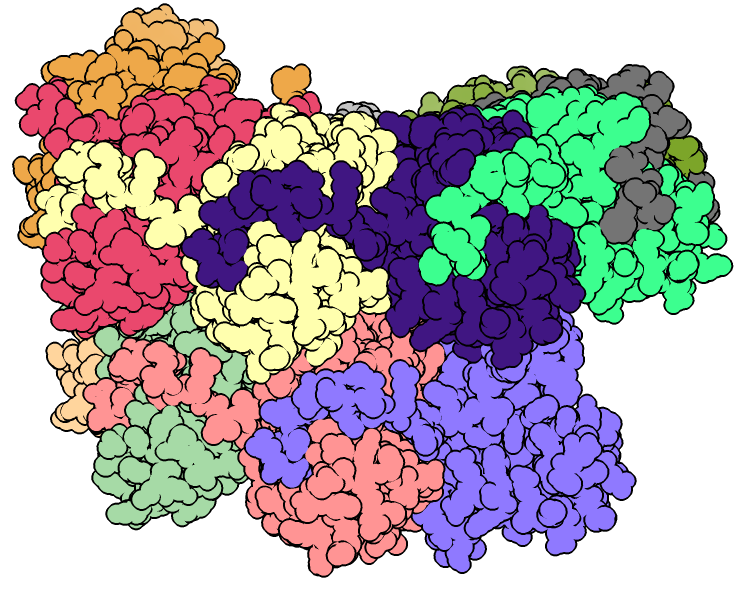
\includegraphics[height=2.5cm]{pvx_slices/vis_helix.png} \\
        \hline
        3x3 & $I=\{0, \pm 1, \pm 8, \pm 9, \pm 10 \}$ & 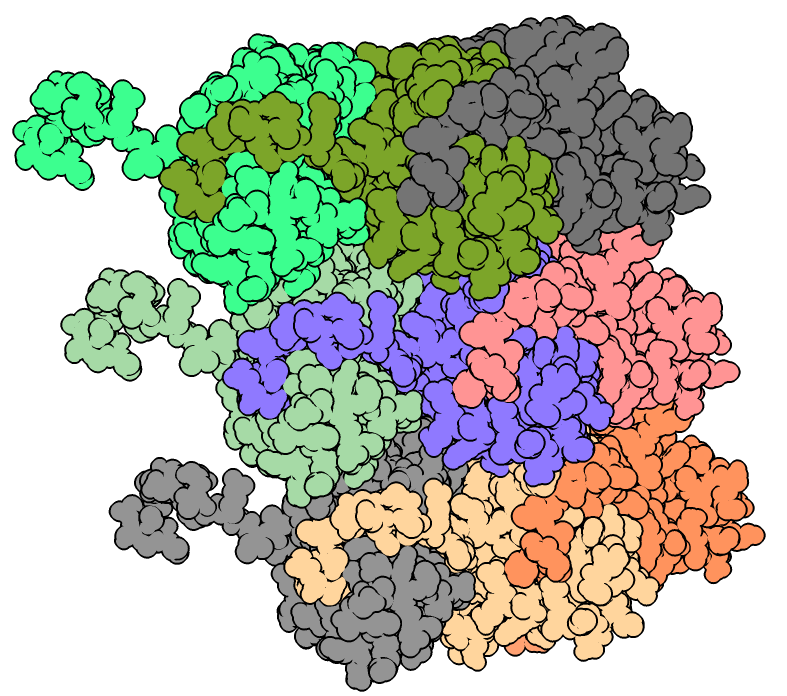
\includegraphics[height=2.5cm]{pvx_slices/vis_3x3.png} \\
        \hline
        Trimer & $I=\{0, \pm 1\}$ & 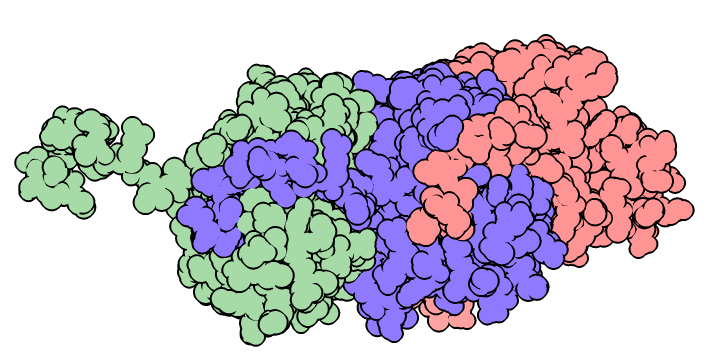
\includegraphics[height=1.5cm]{pvx_slices/vis_trimer.png} \\
        \hline
        Pentamer & $I=\{0, \pm 1, \pm 9 \}$ & 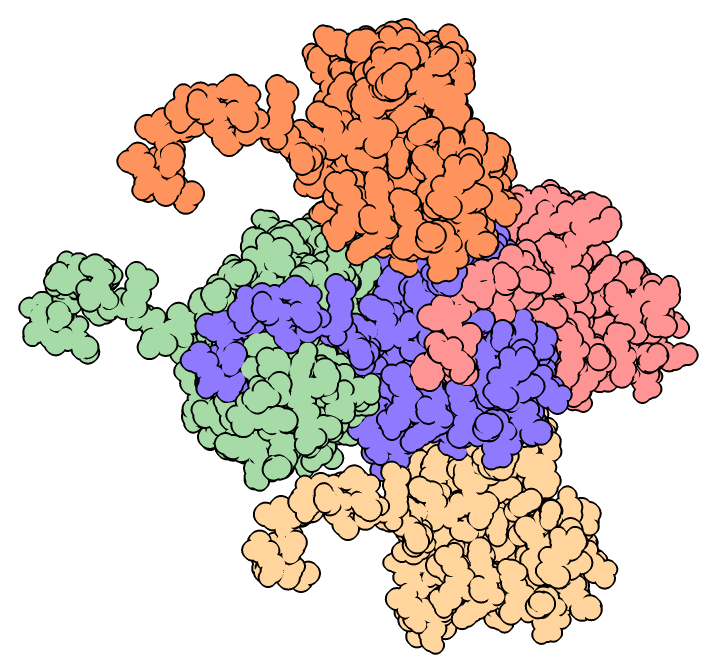
\includegraphics[height=2.5cm]{pvx_slices/vis_pentamer.png} \\
        \hline
    \end{tblr}
    \label{tab:01_symmetry}
\end{table}

Given the relative transform $T_R$, model coordinates can be reconstructed based on the coordinates of the monomer $A$ according to 

\begin{equation}\label{eq:01_symmetry}
\vec{\mathbf{r}}_{j,i}^{\,\text{original}} = T_0 \circ T_R^j \circ \vec{\mathbf{r}}_{A,i}
\end{equation}

Using \autoref{eq:01_symmetry}, four different configurations of monomers are generated and used throughout the following sections (\autoref{tab:01_symmetry}). A helical configuration consisting of thirteen consecutive monomers, a three-by-three neighborhood of nine monomers, a trimer consisting of three consecutive monomers, and a pentamer consisting of five monomers aranged in a cross-shape. 

Despite the small standard deviation of $T_R$, the deviation of individual atom positions in the helical thirteen-monomer reconstruction compared to the data from the pdb entry reaches up to $\SI{0.8}{\angstrom}$. This is due to lever effects caused by small deviations in the rotation. The difference in structure introduces no new clashes, but slightly reduces the contacts by $\SI{2}{\percent}$, as computed with ChimeraX \cite{ChimeraX2023}.
\FloatBarrier

\section{Sequence Design with ProteinMPNN}\label{ch:pmpnn}
ProteinMPNN \cite{PMPNN2022} is a deep learning model for protein sequence design, capable of creating de-novo designs of proteins that fold into a desired shape or bind to specific targets. ProteinMPNN can create sequences for monomers, heterooligomers, and homooligomers. 

The sequence is designed based on a protein backbone as input, that is the position of all backbone atoms of one or multiple chains. The underlying algorithm uses a Message Passing Neural Network (MPNN), a graph-based machine learning model. Each residue in the protein is encoded as a vertex in the graph, and edges are drawn up from each residue to its 48 closest neighbors. Vertex embeddings are initialized as 0 vectors, while the initial edge embeddings are computed based on the distances between the backbone atoms of the residue pair and the difference of their residue indices. After the computation of the initial feature embeddings, ProteinMPNN follows an encoder-decoder architecture, in which the encoder updates the edge and vertex embeddings based on their neighborhood, wheras the decoder uses the embeddings computed by the encoder to predict the amino acid type for each residue. The decoder works in an autoregressive fashion by choosing a random order for decoding the individual residues, then predicting their residue type one-by-one with knowledge of all already predicted residues. Concretely, the algorithm predicts logits $\{\ell_i\}$ for each amino acid and chooses it from a softmax distribution according to
$$P(a_i) = \frac{\exp\left( \frac{\ell_i}{\tau} \right)}{\sum_{j=1}^{20} \exp\left( \frac{\ell_j}{\tau} \right)}$$
Here, $\tau>0$ denotes a chosen temperature constant in the softmax distribution. For $\tau\rightarrow\infty$, the distribution is almost uniform, while for $\tau\rightarrow 0$ the amino acid with the highest predicted logit is chosen. The distribution can be biased by adding to the logits before sampling. For homooligomers, the logits of identical residues in different monomers are averaged and only one amino acid is sampled from the distribution for all of them. 

In this work, all sequences used in computational and experimental evaluation are generated using ProteinMPNN. The input structure is either chosen as the backbone structure of the wildtype, thereby generating alternative sequences for the structure, or a generated artificial backbone as described in \autoref{ch:rfdiffusion}. Of particular note is the choice of the input structure: The helical virus particle consists of approximately 1300 monomers \cite{Grinzato2020}, and truncation to a smaller number will lead to an incorrect neighborhood during featurization for newly exposed residues. 

However, a modification to the original ProteinMPNN algorithm can circumvent this by allowing sequence prediction for a theoretical infinite extension of a symmetric homooligomer. In ProteinMPNN, feature initialization depends solely on the relative neighborhood of each residue, meaning that the initialization is identical for all corresponding residues in a symmetric homooligomer. Further, the message-passing algorithm in the network conserves this equivariance. Therefore, a theoretical infinite extension of the homooligomer can be simulated by remapping of interchain edges to the corresponding residue in the same chain (\autoref{fig:pmpnn_graph}), thereby reducing the input to a single monomer. 

\begin{figure}
\centering
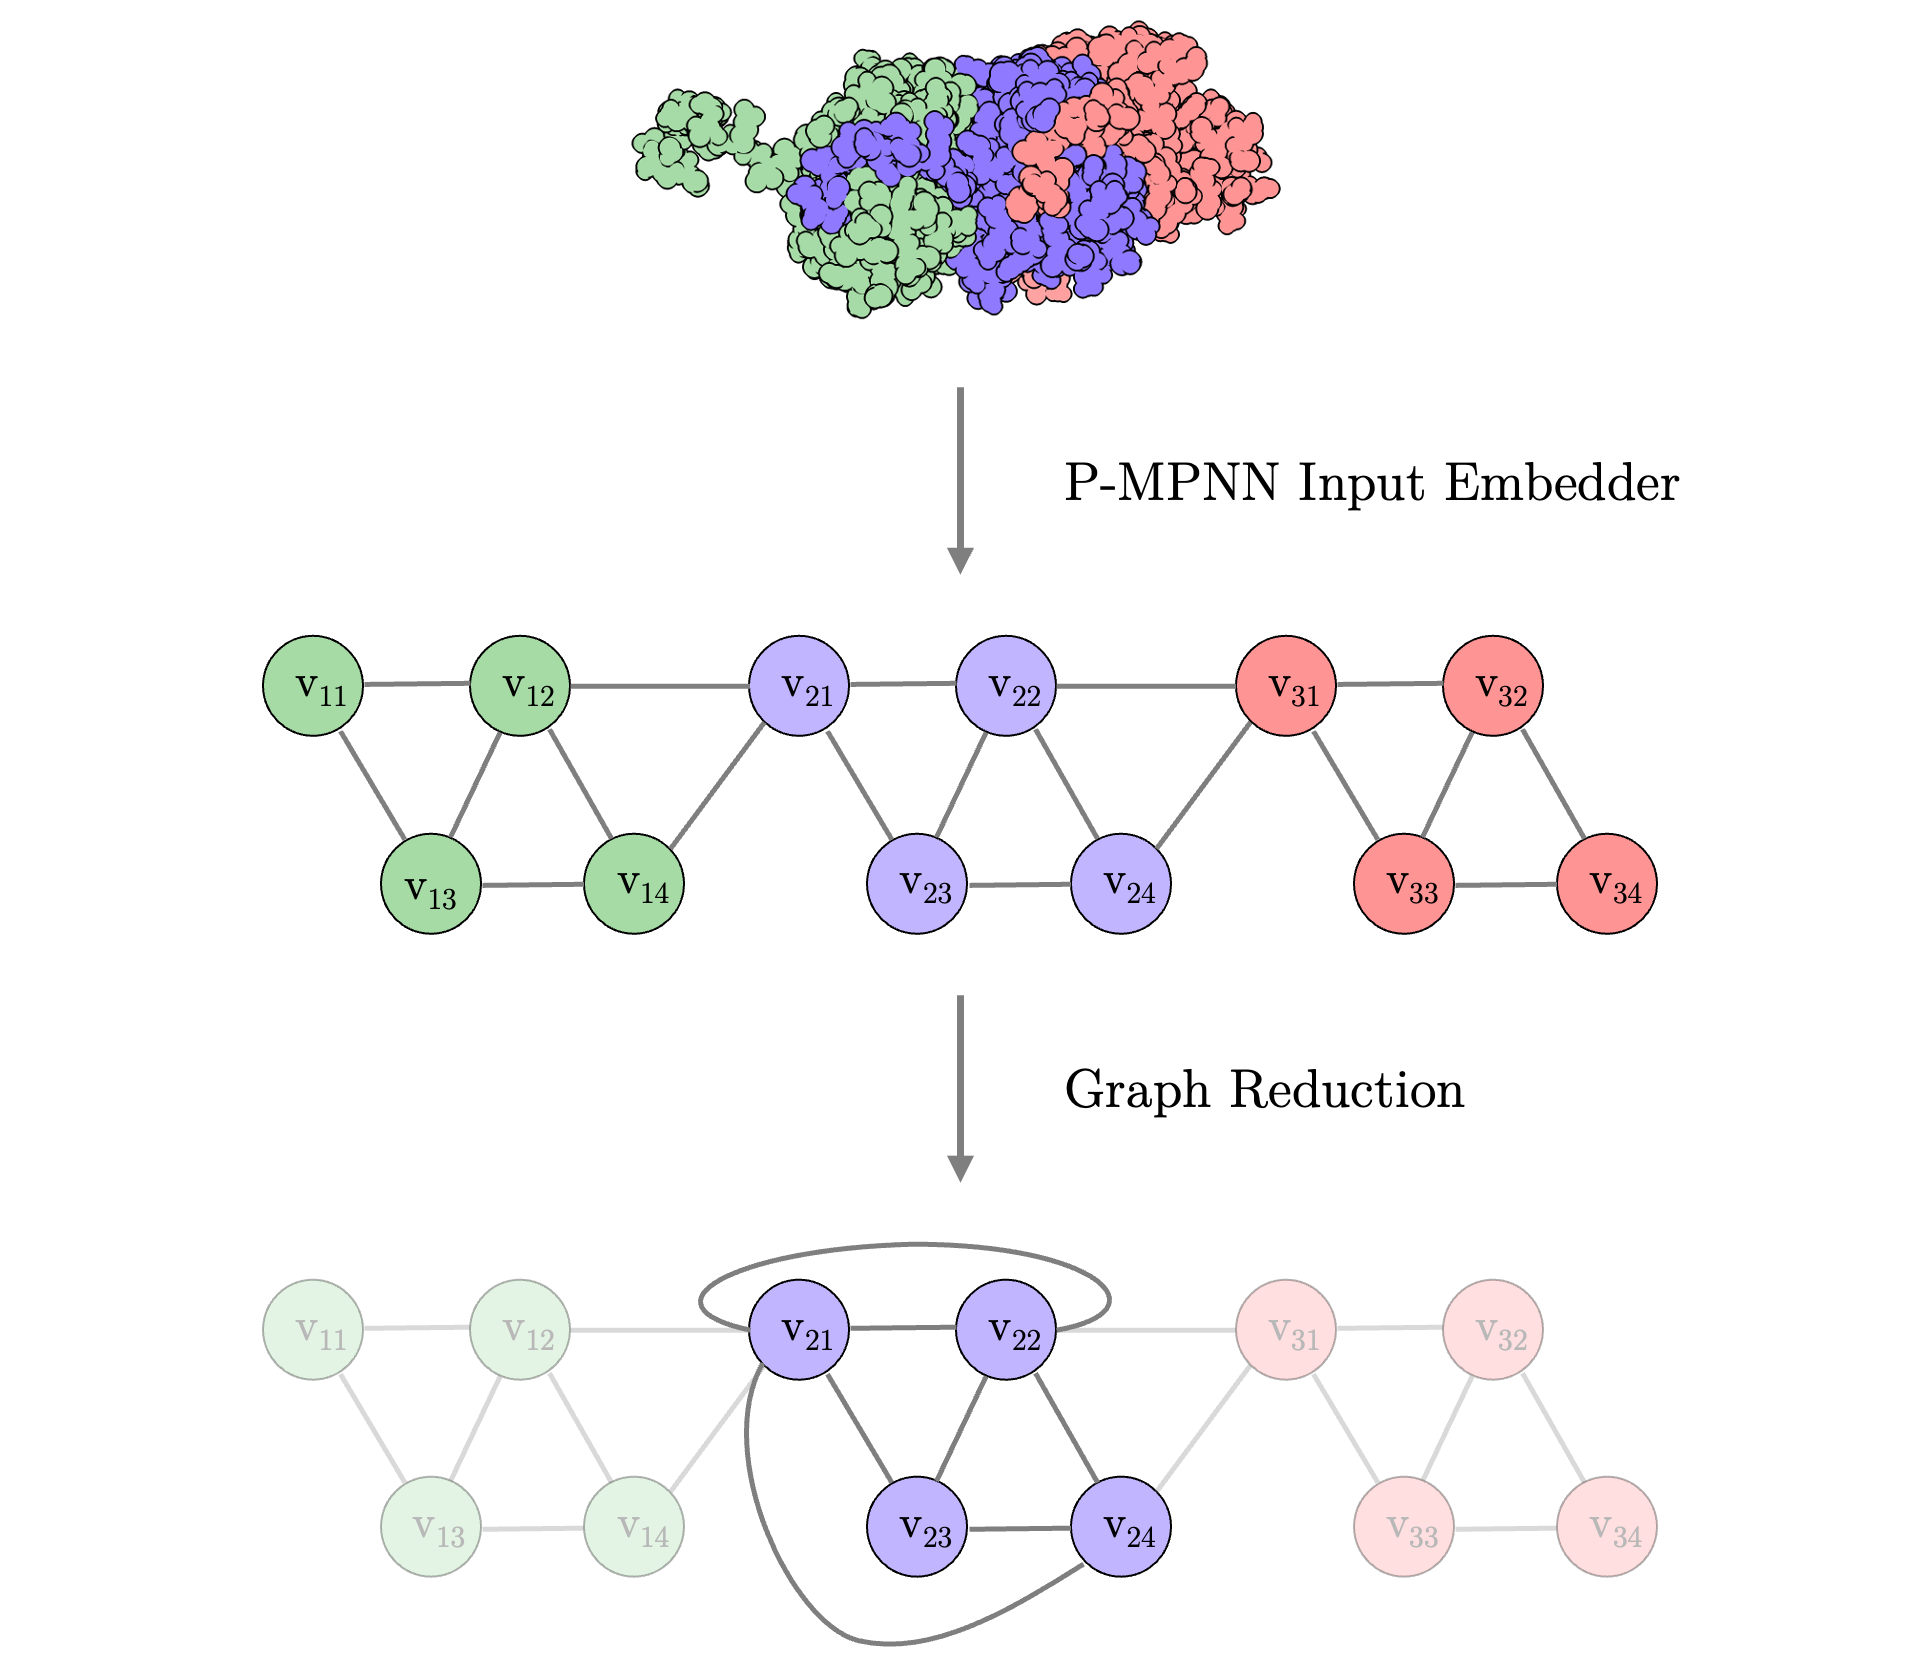
\includegraphics[width=\textwidth]{pmpnn_graph.png}
\caption{\textbf{Graph Reduction procedure for symmetric homooligomers.} After the default graph initialization from ProteinMPNN, one of the monomers is chosen as the reference monomer. Edges going out from it to other monomers are remapped to the corresponding residue in itself. Afterward, vertices and edges of the non-reference monomers are discarded. Through this method, homooligomers with a theoretically infinite geometry can be modeled. }
\label{fig:pmpnn_graph}
\end{figure}

When testing this new algorithm for different helical viruses, the Graph Reduction procedure showed no significant improvement compared to prediction based on a 2x2 neighborhood or a 3x3 neighborhood of monomers (\autoref{fig:pmpnn_comp}). For PVX and Tobacco Mosaic Virus (TMV), the three multimeric inputs (2x2 / 3x3 / infinite neighborhood) performed better than prediction based on a sole monomer, while no such improvement was observed for Pepino Mosaic Virus (PepMV) and Bamboo Mosaic Virus (BaMV) where all methods had similar sequency recovery rates. These results suggest that for the tested proteins, the incorrect neighborhood for small crops doesn't lead to an increased call of wrong amino acids in the aggregated logits. The newly developed infinite symmetry approach performs on par with 2x2 or 3x3 neighborhood prediction, but lowers the amount of required compute to that of a single monomer. However, it is to note that computational cost is generally not a concern when running ProteinMPNN due to its low complexity. 

\begin{figure}
\centering
\includesvg[width=\textwidth]{modeling/pmpnn_comparison.svg}
\caption{\textbf{Sequence recovery by ProteinMPNN for different input configurations.} The input was chosen as either a single monomer, a 2x2 neighborhood, a 3x3 neighborhood, or a symmetry-preserving graph reduction, modeling a theoretical infinite neighborhood. For each of the four targets Potato Virus X (PVX), Tobacco Mosaic Virus (TMV), Pepino Mosaic Virus (PepMV) and Bamboo Mosaic Virus (BaMV), each model was evaluated 50 times using random decoding orders and a sampling temperature $\tau\rightarrow 0$. The errorbars indicate the standard deviation over the repeated evaluation. }
\label{fig:pmpnn_comp}
\end{figure}

ProteinMPNN was used to generate sequences based on the wildtype backbone structure of PVX using the introduced Graph Reduction technique to model an infinite symmetry and a sampling temperature of $\tau\rightarrow 0$, e.g. argmax sampling. Sequences were generated with varying bias $b$ towards the wildtype sequence, that is by increasing the logit of the residue that's present in the wildtype structure by $b$ before sampling the amino acid. For each of the bias values $b \in \{0, 1, 2, 2.5\}$, five sequences were generated. The sequence identity of the generated sequences to the wildtype was about $0.54$ (bias $0$), $0.73$ (bias $1$), $0.88$ (bias $2$) and $0.94$ (bias $2.5$). The generated sequences were further analyzed as described in the \autoref{ch:alphafold} and \autoref{ch:gromacs} before selecting some for experimental evaluation. 
\FloatBarrier

\section{Backbone Design with RFdiffusion}\label{ch:rfdiffusion}
RFdiffusion is a generative machine learning model for protein backbone design. It can be run in different modes to accomplish several tasks such as unconditional monomer generation, protein binder design, scaffolding around a fixed motif, or design of symmetric oligomers (\autoref{fig:rfdiff_trajectories}), the latter being the most relevant for this work. In practice, RFdiffusion is commonly used together with ProteinMPNN, where RFdiffusion generates synthetic backbone structure and ProteinMPNN tries to realize this backbone with a synthetic sequence. 

\begin{figure}
\centering
\includesvg[width=\textwidth]{modeling/rfdiffusion_traj_basic.svg}
\caption{\textbf{RFdiffusion trajectories for unconditional generation and symmetric noise.} For unconditional generation, the RFdiffusion algorithm samples the initial positions independently from a Gaussian distribution and generates the protein without any constraints. For the generation of oligomers with a specific symmetry, RFdiffusion only samples coordinates for one monomer and initializes the other coordinates by applying the respective symmetry transform to the coordinates of that reference monomer. In each diffusion step, this is repeated to enforce the symmetry. }
\label{fig:rfdiff_trajectories}
\end{figure}

Generation by RFdiffusion is performed through a reverse Riemannian diffusion process on the manifold $\mathrm{SE}(3)$. Compared to other diffusion-based algorithms like AlphaFold3 (\autoref{ch:alphafold}), RFdiffusion doesn't operate on the atom coordinates using standard euclidean diffusion, but diffuses the backbone transforms instead. However, it converts the transforms from and to atom coordinates in each iteration. For unconditional generation, the model starts with randomly initialized backbone coordinates and creates a based solely on a specified number of residues. For the creation of symmetric oligomers, the user specifies a set of transforms $\mathfrak{R}=\{R_k\}_{k=1}^K \in \mathrm{SO}(3)$ that define the symmetry. The final protein will satisfy $x^{(k)} = R_k x^{(1)}$, where $x^{(k)}$ denotes the coordinates of the $k$-th monomer. This is achieved by explicitly setting the coordinates as such after initialization and in each further iteration (\autoref{alg:rfdiff}). 

\begin{algorithm}
    \caption{Generation of symmetric oligomers}
    \begin{algorithmic}[1]
    \AlgFunctionDef{SampleSymmetric}{$M, \mathfrak{R} = \{R_k\}_{k=1}^K$}
    \AlgComment{RFdiffusion generation of oligomer with symmetry $\mathfrak{R}$}
    \State $x^{(T,1)} = \text{SampleReference}(M)$
    \ForAll{$t = T, \ldots, 1$}
        \AlgComment[1]{Symmetrize chains}
        \State $X^{(t)} = [R_1 x^{(t,1)}, \ldots, R_K x^{(t,1)}]$
        \State $\hat{X}^{(0)} = \text{RFdiffusion}(X^{(t)})$
        \State $[x^{(t-1,1)}, \ldots, x^{(t-1,K)}] = \text{ReverseStep}(X^{(t)}, \hat{X}^{(0)})$
    \EndFor
    \State \Return $\hat{X}^{(0)}$
    \end{algorithmic}
    \label{alg:rfdiff}
\end{algorithm}

In the original RFdiffusion code, only point group symmetries are supported, that is symmetries that satisfy $\{x^{(1)}, ..., x^{(K)}\} = \{R_j x^{(1)}, ..., R_j x^{(K)}\}$ for each $R_j$, up to reordering of the monomers. Technically, the code could work on general euclidean transforms $T_j \in \mathrm{SE}(3)$ (such as the transforms from \autoref{ch:symmetry} specifying the symmetry of PVX) as well. However, there are certain drawbacks in doing so. The positions in the early steps in the diffusion process follow a Gaussian distribution. While the rotations by point group symmetries conserve that distribution, general euclidean transforms don't. This means that the positions that are fed into the noise prediction network in the diffusion process don't follow the distribution the model is trained on. Further, the authors of RFdiffusion observed that for point group symmetries, the noise prediction model conserves the symmetry almost perfectly. Due to this, the explicit symmetrization in each iteration is generally not necessary and barely affects the trajectory, if the initial noise is symmetrized. This arises from the equivariance of the $\mathrm{SE}(3)$-transformer architecture used in RFdiffusion. Using the symmetry transforms for PVX as evaluated in \autoref{ch:symmetry}, the atom positions in early stages of the diffusion process don't follow a Gaussian distribution, and same-seeded trajectories using either full symmetry enforcement or only initially symmetrized noise differ strongly (\autoref{fig:rfdiff_sym_trajectories}). Rather, for initial symmetrization, the atoms quickly collapse to a Gaussian-like distribution, before spreading out again to form the final multimer.

\begin{figure}[!hbtp]
    \centering
    \includesvg[width=\textwidth]{modeling/rfdiffusion_traj_symmetry.svg}
    \caption{\textbf{RFdiffusion trajectories using the PVX symmetry with full and initial symmetry enforcement. } For initial symmetrization, only the initial Gaussian noise is symmetrized by initializing only one monomer randomly and calculating all other coordinates by applying the symmetry transforms to these reference coordinates. For full symmetrization, this step is repeated at the start of each iteration. While the atom coordinates quickly collapse to a Gaussian-like distribution for only initial symmetrization, full symmetrization forces a separation of the monomer coordinates. }
    \label{fig:rfdiff_sym_trajectories}
\end{figure}

\FloatBarrier

RFdiffusion with full symmetry enforcement of the PVX symmetry was used to generate backbone structures for further testing. In total, five different backbone structures were designed, and ProteinMPNN was used as described in \autoref{ch:pmpnn} to generate five sequences for each of them. Additionally, backbone structures were generated using partial denoising, where only a limited amount of noise was added to the wild type structure before denoising again. This was done using 5, 10, 15, and 20 noise steps in RFdiffusion. For each of these noise levels, three denoised backbones were generated using RFdiffusion, each realized by three sequences through ProteinMPNN. The de novo generated backbones typically consist of a simple structure of alpha helices and beta sheets (\autoref{fig:rfdiffusion_examples}). Possibly due to the aforementioned incongruities in running the algorithm with euclidean transforms, backbone structures generated for the PVX symmetry tended to have structural violations, in particular interchain clashes. The sequences were further evaluated using the methods described in \autoref{ch:alphafold} and \autoref{ch:gromacs}.


\begin{figure}
\centering
\includesvg[width=\textwidth]{modeling/rfdiffusion_examples.svg}
\caption{\textbf{Trimer structures of the PVX wild type CP and designs by RFdiffusion. } The wild type structure (a) was created from the PDB entry by removing all but three monomers. The designs (b) and (c) were created by RFdiffusion using full symmetry enforcement, based on the symmetry transform of PVX. }
\label{fig:rfdiffusion_examples}
\end{figure}


\FloatBarrier

\section{Evaluation with AlphaFold}\label{ch:alphafold}
\begin{algorithm}
    \caption{Sample Diffusion}
    {\small
    \begin{algorithmic}[1]
        \AlgFunctionDef{SampleDiffusion}{$\{\mathbf{f}^*\}$, $\{\mathbf{s}_i^{\text{inputs}}\}$, $\{\mathbf{s}_i^{\text{trunk}}\}$, $\{\mathbf{z}_{ij}^{\text{trunk}}\}$, Noise Schedule $[c_0, c_1, \ldots, c_T]$, $\gamma_0 = 0.8$, $\gamma_{\min} = 1.0$, noise scale $\lambda = 1.003$, step scale $\eta = 1.5$}
        \State $\vec{\mathbf{x}}_l \sim c_0 \cdot \mathcal{N}(\vec{\mathbf{0}}, \mathbf{I}_3)$ \hfill $\vec{\mathbf{x}}_l \in \mathbb{R}^3$
        \ForAll{$c_\tau \in [c_1, \ldots, c_T]$}
            \State $\{\vec{\mathbf{x}}_l\} \gets \CustomFunction{\text{CentreRandomAugmentation}}(\{\vec{\mathbf{x}}_l\})$
            \State $\gamma \gets \gamma_0 \text{ if } c_\tau > \gamma_{\min} \text{ else } 0$
            \State $\hat{t} \gets c_{\tau-1}(\gamma + 1)$
            \State $\vec{\boldsymbol{\xi}}_l \gets \lambda \sqrt{\hat{t}^2 - c_{\tau-1}^2} \cdot \mathcal{N}(\vec{\mathbf{0}}, \mathbf{I}_3)$ \hfill $\vec{\boldsymbol{\xi}}_l \in \mathbb{R}^3$
            \State $\vec{\mathbf{x}}_l^{\text{noisy}} \gets \vec{\mathbf{x}}_l + \vec{\boldsymbol{\xi}}_l$
            \State $\{\vec{\mathbf{x}}_l^{\text{denoised}}\} \gets \CustomFunction{\text{DiffusionModule}}(\{\vec{\mathbf{x}}_l^{\text{noisy}}\}, \hat{t}, \{\mathbf{f}^*\}, \{\mathbf{s}_i^{\text{inputs}}\}, \{\mathbf{s}_i^{\text{trunk}}\}, \{\mathbf{z}_{ij}^{\text{trunk}}\})$
            \State $\vec{\boldsymbol{\delta}}_l \gets (\vec{\mathbf{x}}_l - \vec{\mathbf{x}}_l^{\text{denoised}})/\hat{t}$
            \State $dt \gets c_\tau - \hat{t}$
            \State $\vec{\mathbf{x}}_l \gets \vec{\mathbf{x}}_l^{\text{noisy}} + \eta \cdot dt \cdot \vec{\boldsymbol{\delta}}_l$
        \EndFor
        \State \textbf{return} $\{\vec{\mathbf{x}}_l\}$
        \end{algorithmic}
    }
\end{algorithm}


\begin{algorithm}
    \caption{Sample Diffusion\algHighlight{ with Symmetrization for Multimeric Complexes}}
    {\small
    \begin{algorithmic}[1]
        \AlgFunctionDef{SampleDiffusion}{$\{\mathbf{f}^*\}$, $\{\mathbf{s}_i^{\text{inputs}}\}$, $\{\mathbf{s}_i^{\text{trunk}}\}$, $\{\mathbf{z}_{ij}^{\text{trunk}}\}$, Noise Schedule $[c_0, c_1, \ldots, c_T]$, $\gamma_0 = 0.8$, $\gamma_{\min} = 1.0$, noise scale $\lambda = 1.003$, step scale $\eta = 1.5$, \algHighlight{Monomer Transforms $\{T_j\}$, Monomer Indices $\{I_j\}$}}
        \State $\vec{\mathbf{x}}_l \sim c_0 \cdot \mathcal{N}(\vec{\mathbf{0}}, \mathbf{I}_3)$ \hfill $\vec{\mathbf{x}}_l \in \mathbb{R}^3$
        \AlgComment{Modification: Initial Symmetrization}
        \AlgCustomLine{$(R_{\text{ref}}, \vec{\mathbf{t}}_{\text{ref}}) \gets (\mathbf{I}, \text{mean}(\{\vec{\mathbf{x}}_l\}_{l \in I_1}))$} \hfill Denoted as $T_{\text{ref}}=(R_{\text{ref}}, \vec{\mathbf{t}}_{\text{ref}})$
        \AlgCustomLine{\textbf{for all} $j \in [2, \ldots, N_{\text{monomer}}]$}
            \AlgCustomLine[1]{ $\{\vec{\mathbf{x}}_l\}_{l \in I_j} \gets T_{\text{ref}} \circ T_j \circ T_{\text{ref}}^{-1} \circ \{\vec{\mathbf{x}}_l\}_{l \in I_1}$}
        \AlgCustomLine{\textbf{end for}}
        
        \ForAll{$c_\tau \in [c_1, \ldots, c_T]$}
            \AlgComment[1]{Track Origin of Symmetrization Center}
            \AlgCustomLine[1]{$\vec{\mathbf{t}}_{\text{ref}} \gets \text{mean}(\{\vec{\mathbf{x}}_l\}_{l \in I_1})$}
            \State $\{\vec{\mathbf{x}}_l\}$\algHighlight{, $T_{\text{aug}}$}$ \gets \CustomFunction{\text{CentreRandomAugmentation}}(\{\vec{\mathbf{x}}_l\})$
            \AlgComment[1]{Track Movement by CentreRandomAugmentation}
            \AlgCustomLine[1]{$T_{\text{ref}} \gets T_{\text{aug}} \circ T_{\text{ref}}$}
            
            \State $\gamma \gets \gamma_0 \text{ if } c_\tau > \gamma_{\min} \text{ else } 0$
            \State $\hat{t} \gets c_{\tau-1}(\gamma + 1)$
            \State $\vec{\boldsymbol{\xi}}_l \gets \lambda \sqrt{\hat{t}^2 - c_{\tau-1}^2} \cdot \mathcal{N}(\vec{\mathbf{0}}, \mathbf{I}_3)$ \hfill $\vec{\boldsymbol{\xi}}_l \in \mathbb{R}^3$
            \State $\vec{\mathbf{x}}_l^{\text{noisy}} \gets \vec{\mathbf{x}}_l + \vec{\boldsymbol{\xi}}_l$
            
            \State $\{\vec{\mathbf{x}}_l^{\text{denoised}}\} \gets \CustomFunction{\text{DiffusionModule}}(\{\vec{\mathbf{x}}_l^{\text{noisy}}\}, \hat{t}, \{\mathbf{f}^*\}, \{\mathbf{s}_i^{\text{inputs}}\}, \{\mathbf{s}_i^{\text{trunk}}\}, \{\mathbf{z}_{ij}^{\text{trunk}}\})$
            
            \AlgComment[1]{Recenter and Symmetrize Denoised Prediction}
            \AlgCustomLine[1]{$\vec{\mathbf{x}}_l^{\text{denoised}} \mathrel{+}= \text{mean}(\{\vec{\mathbf{x}}_l^{\text{noisy}}\}_{l \in I_1}) - \text{mean}(\{\vec{\mathbf{x}}_l^{\text{denoised}}\}_{l \in I_1})$}
            \AlgCustomLine[1]{\textbf{for all} $j \in [2, \ldots, N_{\text{monomer}}]$}
                \AlgCustomLine[2]{$\{\vec{\mathbf{x}}_l^{\text{denoised}}\}_{l \in I_j} \gets T_{\text{ref}} \circ T_j \circ T_{\text{ref}}^{-1} \circ \{\vec{\mathbf{x}}_l^{\text{denoised}}\}_{l \in I_1}$}
            \AlgCustomLine[1]{\textbf{end for}}
        
            \State $\vec{\boldsymbol{\delta}}_l \gets (\vec{\mathbf{x}}_l - \vec{\mathbf{x}}_l^{\text{denoised}})/\hat{t}$
            \State $dt \gets c_\tau - \hat{t}$
            \State $\vec{\mathbf{x}}_l \gets \vec{\mathbf{x}}_l^{\text{noisy}} + \eta \cdot dt \cdot \vec{\boldsymbol{\delta}}_l$
        \EndFor
        \State \textbf{return} $\{\vec{\mathbf{x}}_l\}$
        \end{algorithmic}
    }
    \end{algorithm}
\FloatBarrier

\section{Evaluation with GROMACS}\label{ch:gromacs}
% Further evaluation through GROMACS: 
% Physics based evaluation by Cao et al (physics_binder_design)
% Physics based evaluations generally perform worse than AI for AI designs (binder_design)
% However, important metric because we used AI off from the tested setup
% For viruses, all-atom MD Simulations used widely for structural analysis tasks
% md_viral_analysis_review
% in particular md_tmv_stability for assessing stability in absence of RNA
% similar for us: simulation of a slice with 13 particles, RMSD shift
% three designs with intermediate structural stability. RFdiffusion samples
% immediately went really high
% notably: starting with predicted Wildtype structure, stability can be partly recovered,
% then similar to the designs
For further in silico evaluation of the designs, Molecular Dynamics (MD) simulations using GROMACS \cite{gromacs_general} were conducted. Similar physics based evaluations have already been proven to be a suitable metric for assessing the quality of novel binder designs \cite{physics_binder_design}. While physics based metrics tended to be less effective for design evaluation than methods based on AlphaFold \cite{binder_design}, the metric might be particularly viable for the designs created in this work, since the methods of symmetry-guided design (\autoref{ch:rfdiffusion}) and symmetry-guided prediction (\autoref{ch:alphafold}) might introduce a bias for the AI tools. 

For viruses, all-atom MD simulations are widely used for several tasks regarding structural analysis and assembly \cite{md_viral_analysis_review}. In particular, Freddolino et al. were able to analyze structural integrity of Satellite Tobacco Mosaic Virus  (STMV), showing that the capsid becomes unstable in absence of RNA \cite{md_tmv_stability}. This instability was observed as an increase in the RMSD of the viral atoms compared to the initial structure over the course of the simulation. 

A similar trend was observed in this work as well. In MD simulations of a slice of 13 monomers at a temperature of \SI{310}{\kelvin} (also conducted at \SI{300}{\kelvin with similar results}), RMSD for the wild type excluding RNA increased significantly quicker than for the wild type with its genomic RNA included (\autoref{fig:gromacs_rmsd_gyrate}). Three of the artificial designs showed an RMSD development in-between these two, while the designs based on RFdiffusion quickly rose to RMSDs more than twice as large as that of the wild type without RNA (data not shown), likely due to the observed structural violations in the designs. Notably, when running the simulation of the wild type without RNA based on an initial guess by AlphaFold instead of the PDB structure, the RMSD progresses similar to those of the artificial designs.

\begin{figure}
    \includesvg{modeling/gromacs_joined_rmsd_gyrate_plot.svg}
    \caption{\textbf{Evolution of RMSD from the initial structure throughout a GROMACS simulation. } The Designs A, B, and C were generated with ProteinMPNN based on the wild type PVX CP structure with varying bias towards the wild type sequence. The predicted wild type structure was selected similar to the designs, as the prediction closest to the wild type in C$\alpha$-RMSD out of five symmetry-enforced AlphaFold predictions. The lines indicate the RMSD after smoothing with a Savitzky-Golay filter with a windowsize of \SI{0.5}{\nano\second}, while the colored areas show the running standard deviation over that window. The RMSD of the RFdiffusion designs was significantly larger and is not shown. }
    \label{fig:gromacs_rmsd_gyrate}
\end{figure}

% Further: ddG analysis proved up as a helpful metric for binder design
% might help here as well: Assessment of binding enthalpy using umbrella sampling and the 
% WHAM method wham_method
% free energy of binding estimate of 165 kcal/mol Design A
% slightly higher than wildtype 160kcal/mol
% Design B and C lower binding energy estimates of 120 and 115 kcal/mol
% Predicted wildtype significantly worse here: only 105 kcal/mol
% High impact by initial conditions
% not perfect: not conducted in equilibrium, pulling was too strong
% reason: problems with unraveling, more complex pull coordinates might help
% Selection of designs: Design A and Design B, Design A both with and without S-Tag, Design B only with S-Tag
In the context of binder design, another metric that proved to be an effective predictor was the Rosetta ddG estimate of the complex's free binding energy \cite{physics_binder_design}. Similar free energy simulations can also be conducted in GROMACS using Umbrella Sampling and the Weighted Histogram Analysis Method (WHAM) \cite{wham_method}. Here, an estimate of the binding energy is calculated by forcing the proteins apart from each other using a moving potential, then running simulations along intermediate steps of the trajectory. The binding energy can be computed from these simulations through estimating the thermodynamical likelihood $P(x)$ of each distance. Concretely, the potential of mean (the free energy along the pulling coordinate) can be computed as 
\begin{equation}
    F(x) = -k_B T \log(P(x)) + C
\end{equation}

where $k_B$ is the Boltzmann constant, T is the temperature, C is a constant offset, and $P(x)$ is the probability distribution over the distance $x$ between the monomers. The free binding energy is then the difference of the potential of mean force in the unbound and the bound state. 

The free binding energy was calculated for the wild type and three of the designs (\autoref{fig:gromacs_pmf}). The free energy estimate for Design A of \SI{165}{\kilo\cal\per\mole} was slightly higher than that of the wild type of \SI{160}{\kilo\cal\per\mole}. Designs B and C were evaluated to lower binding energies of \SI{120}{\kilo\cal\per\mole} and \SI{115}{\kilo\cal\per\mole}. Calculation of the free energy based on the predicted initial structure of the wild type instead of the PDB structure lead to a binding energy of only \SI{105}{\kilo\cal\per\mole}. This is significantly lower than the value based on the PDB structure, even though the two models only have an RMSD of \SI{0.9}{\angstrom}. This suggests a strong dependence of the calculation on the initial state of the system. The computed binding energies are comparable in magnitude to a reported \SI[separate-uncertainty=true]{-144.9(4.9)}{\kilo\cal\per\mole} dimerization energy for the coat proteins of Cowpea Chlorotic Mottle Virus \cite{ccmv_binding_energy}. The free energy calculations were conducted at relatively high pulling rates, which is generally discouraged since it can create unrealistic dissociation pathways that hinder PMF estimation \cite{lemkul_umbrella_sampling}, \cite{umbrella_sampling_problems}. The high pulling rates were chosen because the proteins tended to unravel in the simulations using lower pulling rates, and the required simulation size for full dissociation would have exceeded the computational resources available for this project. As a result, the estimated binding energies should be interpreted with caution, as they may not fully reflect the true thermodynamic values.

\begin{figure}
    \includesvg{modeling/gromacs_wham_profile.svg}
    \caption{\textbf{Estimated Potential of Mean Force along the dissociation coordinate} of homodimers for the ProteinMPNN designs A, B, and C, as well as the wild type structure from the PDB and the predicted wild type structure. The PMF was calculated using Umbrella Sampling and the WHAM method. The simulations were conducted with high pulling rates, which can negatively impact the results. }
    \label{fig:gromacs_pmf}
\end{figure}

Based on the simulations, designs A and B were chosen for experimental evaluation in the laboratory. As mentioned earlier, the structural design was based on the d29-PVX-CP, since the structure of the flexible tail is not determined. Given the relevance of the N-terminal domain for the wild type structure of PVX \cite{del22_rigid}, both designs were prepended with the N-terminal domain of the wild type. Design B only shares \SI{53}{\percent} sequence identity with the PVX CP. Due to this, anti-PVX antibodies might not bind to this design. Based on experience at the Institute of Molecular Biotechnology, an S-Tag was chosen as an N-terminal marker, because it was known to not hinder assembly of PVX, and because it is detectable by an anti-S-Tag antibody. The three designs chosen for laboratory evaluation are thus S-Tag-A, S-Tag-B, and d29-A, the latter being the sequence of design A without any N-terminal modifications. The protein sequences were codon optimized for use in \emph{Nicotiana tabacum} as a host organisms. The designed protein and DNA sequences are described in \autoref{appendix:synthetic_seqs}.
\FloatBarrier

\part{Experimental Evaluation}
\section{Materials}\label{ch:materials}
\subsection{Laboratory Equipment}
% 
\newcolumntype{L}[1]{>{\RaggedRight}p{#1}}
\newcolumntype{M}[1]{>{\raggedright\arraybackslash}p{#1}}
\newcolumntype{P}[1]{>{\hspace{0pt}}p{#1}}
\subsection{Chemicals}
\subsection{Media, Buffers, and Solutions}
All media, buffers, and solutions that were used in the experiments are shown in \autoref{tab:materials_media}. NaOH and HCl were used to establish the pH. 
\begin{longtable}{@{} l l l @{}}
    \caption{\textbf{Media, buffers, and solutions that were used in this study}. Listed are the component types their respective amounts.} \label{tab:materials_media} \\
        \toprule
        \textbf{Medium/buffer/solution} & \textbf{Component} & \textbf{Amount} \\
        \midrule
        \endfirsthead
        \toprule
        \textbf{Medium/buffer/solution} & \textbf{Component} & \textbf{Amount} \\
        \midrule
        \endhead
        agarose gel & Agarose & \SI{1.2}{\percent} (w/v) \\
                        & Ethidium bromide & \SI{0.5}{\micro\gram\per\milli\litre} \\
                        & in 1x TAE buffer & \\[1ex]
        
        AP buffer (pH 9.6) & Tris-HCl & \SI{100}{\milli\Molar} \\
                           & NaCl & \SI{100}{\milli\Molar} \\
                           & MgCl\textsubscript{2} & \SI{5}{\milli\Molar} \\[1ex]
        blocking solution & powedered milk & \SI{40}{\gram\per\litre} \\
                    & in PBS buffer & \\[1ex]
        Coomassie staining solution & Coomassie Brilliant Blue & \SI{2.5}{\gram\per\litre} \\
                                    & Methanol & \SI{50}{\percent} (v/v) \\
                                    & Acetic acid & \SI{10}{\percent} (v/v) \\[1ex]
        coating buffer (pH 9.6) & --- & --- \\
        destaining solution & Methanol & \SI{5}{\percent} (v/v) \\
                            & Acetic acid & \SI{7.5}{\percent} (v/v) \\[1ex]
        elisa substrate solution & --- & --- \\[1ex]
        LB medium & Yeast extract & \SI{5}{\gram\per\litre} \\
                  & Tryptone & \SI{10}{\gram\per\litre} \\
                  & NaCl & \SI{171}{\milli\Molar} \\
                  & (Agar) & \SI{15}{\gram\per\litre} \\[1ex]
        LB-Amp medium & Yeast extract & \SI{5}{\gram\per\litre} \\
                  & Tryptone & \SI{10}{\gram\per\litre} \\
                  & NaCl & \SI{171}{\milli\Molar} \\
                  & Ampicillin & \SI{100}{\milli\gram\per\litre} \\
                  & (Agar) & \SI{15}{\gram\per\litre} \\[1ex]
        NBT/BCIP staining solution & NBT & \SI{33.3}{\gram\per\litre} \\
                                   & BCIP & \SI{16.5}{\gram\per\litre} \\
                                   & in dimethylformamide & \\[1ex]
        PBS buffer & NaCl & \SI{137}{\milli\Molar} \\
              KCl     & \SI{2.7}{\milli\Molar}  \\
              Na\textsubscript{2}HPO\textsubscript{4} & \SI{8.1}{\milli\Molar} \\
              KH\textsubscript{2}PO\textsubscript{4} & \SI{1.5}{\milli\Molar} \\[1ex]

              phosphate buffer (0.01 M, pH 7.2) & Na\textsubscript{2}HPO\textsubscript{4} & \SI{6.67}{\milli\Molar} \\
                                  & NaH\textsubscript{2}PO\textsubscript{4} & \SI{3.33}{\milli\Molar} \\[1ex]
        reducing loading buffer (5x) & Tris-HCl (pH 6.8) & \SI{62.5}{\milli\Molar} \\
                                     & Glycerine & \SI{300}{\gram\per\litre} \\
                                     & SDS & \SI{40}{\gram\per\litre} \\
                                     & $\beta$-Mercaptoethanol & \SI{10}{\percent} (v/v) \\
                                     & Bromophenol blue & \SI{0.1}{\gram\per\litre} \\[1ex]
        Sabu (10x) & Glycine & \SI{50}{\percent} (v/v) \\
                   & Xylene cyanol FF & \SI{0.1}{\percent} (w/v) \\
                   & Bromophenol blue & \SI{0.1}{\percent} (w/v) \\
                   & in 1x TAE buffer (pH 8.0) & \\[1ex]
        SDS running buffer & Glycine & \SI{200}{\milli\Molar} \\
                              & SDS & \SI{1}{\gram\per\litre} \\
                              & Tris & \SI{25}{\milli\Molar} \\[1ex]
        semi-dry transfer buffer & Glycine & \SI{391}{\milli\Molar} \\
                                & Methanol & \SI{20}{\percent} (v/v) \\
                                & Tris & \SI{48}{\milli\Molar} \\[1ex]
        TAE buffer & Tris & \SI{40}{\milli\Molar} \\
                      & Acetic acid & \SI{0.1}{\percent} (v/v) \\
                      & EDTA (pH 8.0) & \SI{1}{\milli\Molar} \\
        \bottomrule
\end{longtable}
\FloatBarrier
\subsection{Reaction Kits}

The following reaction kits were used in this study:
\begin{itemize}
    \item Gibson Assembly\textsuperscript{\textregistered} Cloning Kit, NEB, Ipswich, MA
    \item Mix2Seq Kit, Eurofins Genomics, Ebersberg, Germany
    \item PureYield\textsuperscript{\texttrademark} Plasmid Miniprep System, Promega, Madison, WI
    \item Wizard\textsuperscript{\textregistered} SV Gel and PCR Clean-Up System, Promega, Madison, WI
    \item NucleoBond Xtra Midi kit for transfection-grade plasmid DNA, Macherey-Nagel, Düren, Germany
    \item ALiCE\textsuperscript{\textregistered} for Research kit, LenioBio, Düsseldorf, Germany
  \end{itemize}
\FloatBarrier
\subsection{Enzymes}
All enzymes used in this study are shown in \autoref{tab:materials_enzymes}. 
\begin{table}[h]
    \centering
    \caption{\textbf{Polymerases and restriction enzymes that were used in this study.} Listed are the reagent names, the manufacturer, and how the enzymes were used in the experiments. }
    \begin{tabular}{lll}
    \toprule
    \textbf{Reagent} & \textbf{Manufacturer} & \textbf{Use} \\
    \midrule
    GoTaq\textsuperscript{\textregistered} G2 DNA Polymerase & Promega & Colony PCR \\
    Pfu DNA Polymerase & Promega & Insert Amplification \\
    NcoI-HF\textsuperscript{\textregistered} & NEB & Restriction \\
    KpnI-HF\textsuperscript{\textregistered} & NEB & Restriction \\
    \bottomrule
    \end{tabular}
    \label{tab:materials_enzymes}
\end{table}

\FloatBarrier

\subsection{Plasmids}
\subsubsection{pLenEx-Strep-eYFP}
The plasmid pLenEx-Strep-eYFP was used for cell-free expression of Strep-eYFP using the ALiCE\textsuperscript{\textregistered} expression kit. The plasmid contains an origin of replication for \emph{E. coli}, a gene for ampicillin resistance, and a gene encoding Strep-eYFP. This gene is flanked by 5'- and 3'-UTRs from tobacco mosaic virus (TMV) and under the T7 promoter. The plasmid contains restriction sites for NcoI at the 5' end of Strep-eYFP and for KpnI at the 3' end. In addition to cell-free expression, pLenEx-Strep-eYFP was used for cloning of the genetic elements d29-A, S-Tag-A, and S-Tag-B. The plasmid was provided by the Institute for Molecular Biotechnology.

\subsubsection{pLenEx-d29-A, pLenEx-S-Tag-A, pLenEx-S-Tag-B}
Like pLenEx-Strep-eYFP, the plasmids pLenEx-d29-A, pLenEx-S-Tag-A, and pLenEx-S-Tag-B contain an origin of replication for \emph{E. coli} and a gene for ampicillin resistance. Instead of Strep-eYFP, the vectors carry the genetic elements d29-A, S-Tag-A, and S-Tag-B, as described in \autoref{ch:gromacs}, respectively. These genes are again flanked by 5'- and 3'-UTRs from TMV and are under control of the T7 promoter and in-between the NcoI and KpnI restriction sites. The plasmids were created based on pLenEx-Strep-eYFP using Gibson Assembly.


\subsubsection{pLenEx-CP-PVX}
The plasmid pLenEx-CP-PVX carries the same genetic elements as pLenEx-Strep-eYFP, except for the Strep-eYFP gene, which is instead replaced by a gene encoding for the PVX coat protein. The plasmid was provided by the Institute for Molecular Biotechnology.
\FloatBarrier
\subsection{Antibodies}
%Rabbit-Anti-PVX, polyclonal rabbit IgG, DSMZ AS-0126
%S-peptide Epitope Tag Monoclonal Antibody, monoclonal mouse IgG, Invitrogen MA1-981
%Goat-Anti-Rabbit FC AP, polyclonal goat IgG, coupled with alkaline phosphatase, AffiniPure Jackson Research, UK
%Goat-Anti-Mouse FC AP, polyclonal goat IgG, coupled with alkaline phosphatase, AffiniPure Jackson Research, UK
All antibodies that were used in this study are listed in \autoref{tab:materials_antibodies}. The antibodies were used both for Western Blotting and for ELISA assays. 
\begin{table}[h]
    \centering
    \caption{\textbf{Antibodies that were used in this study.} Listed are the characteristics of the antibody and its manufacturer. }
    \begin{tabular}{lll}
    \toprule
    \textbf{Antibody} & \textbf{Type} & \textbf{Manufacturer / Catalog} \\
    \midrule
    Rabbit-Anti-PVX & Polyclonal rabbit IgG & DSMZ AS-0126 \\
    S-peptide Epitope Tag Monoclonal Antibody & Monoclonal mouse IgG & Invitrogen MA1-981 \\
    Goat-Anti-Rabbit (GAR\textsuperscript{AP}\textsubscript{FC}) & Polyclonal goat IgG, alkaline phosphatase conjugate & Biozol, Hamburg \\
    Goat-Anti-Mouse (GAM\textsuperscript{AP}\textsubscript{FC}) & Polyclonal goat IgG, alkaline phosphatase conjugate & Biozol, Hamburg \\
    \bottomrule
    \end{tabular}
    \label{tab:materials_antibodies}
\end{table}
\FloatBarrier
% TODO: Ask Caro on Antibodies
\subsection{Synthetic Oligonucleotides}
All syntehtic oligonucleotides that were used in this study are shown in \autoref{tab:materials_oligos}. 
\begin{table}[h]
    \centering
    \caption{\textbf{Synthetic oligonucleotides that were used in this study.} Regions overlapping with the amplified genes are displayed in uppercase. }
    \begin{tabularx}{\linewidth}{lXl}
    \toprule
    \textbf{Name} & \textbf{Sequence (5' $\rightarrow$ 3')} & \textbf{Use} \\
    \midrule
    d29-A fwd & acattttacattctacaactaccATGGCTT\newline CTGGCTTATTCACCATACCTG & Insert amplification \\[1ex]
    d29-A rev & ccaaaccagaagagcttggtaccTTAAGGG\newline GGGGGAATGGTCAC & Insert amplification \\[1ex]
    S-Tag-A fwd & acattttacattctacaactaccatggcTA\newline AAGAAACAGCCGCCGCTAAATTC & Insert amplification \\[1ex]
    S-Tag-B fwd & acattttacattctacaactaccatggctA\newline AGGAGACTGCTGCAGCCAAG & Insert amplification \\[1ex]
    S-Tag-B rev & ccaaaccagaagagcttggtaccTTAAGCT\newline GCGGGTATGTGTATGATTC & Insert amplification \\[1ex]
    pLenSeq fwd & \% TODO: Ask Juliane, sequence missing & Sequencing \\[1ex]
    pLenSeq rev & \% TODO: sequence missing & Sequencing \\
    \bottomrule
    \end{tabularx}
    \label{tab:materials_oligos}
\end{table}
\FloatBarrier

\subsection{Synthetic Genes}\label{subseq:synthetic_genes}
Genes for the constructs S-Tag-A and S-Tag-B were ordered from Integrated DNA Technologies (Coralville, Iowa). The exact sequences can be found in \autoref{appendix:synthetic_seqs}.

\subsection{Organisms}
NEB\textsuperscript{\textregistered} Turbo Competent \emph{E. coli} (High Efficiency) was used for cloning of the plasmids pLenEx-d29-A, pLenEx-S-Tag-A, and pLenEx-S-Tag-B.

\section{Methods}\label{ch:methods}
\subsection{DNA Cloning}
\subsubsection{PCR Amplification of Insert DNA}
Using the synthetic genes S-Tag-A and S-Tag-B (Subsection \ref{subseq:synthetic_genes}) and the primer pairs d29-A fwd / d29-A rev (with template S-Tag-A), S-Tag-A fwd / d29-A rev (with template S-Tag-A), and S-Tag-B fwd / S-Tag-B rev (with template S-Tag-B), polymerase chain reactions (PCRs) were conducted for amplification of the inserts. The primers also introduced overlapping regions with the plasmid pLenEx-Strep-eYFP for the following Gibson Assembly, and in the case of d29-A fwd, a start codon. The PCR was conducted with a Pfu polymerase. The composition of the PCR mix is listed in Table \ref{tab:methods_pcr_composition}.
\begin{table}
    \centering
    \caption{\textbf{Composition of the PCR Mix for Insert Amplification. }}
    \label{tab:methods_pcr_composition}
\begin{tabular}{ll}
\toprule
\textbf{Component} & \textbf{Amount} \\
\midrule
MQ-H\textsubscript{2}O & \SI{38}{\micro\litre} \\
10x Pfu Buffer & \SI{5}{\micro\litre} \\
dNTPs ($\SI{10}{\milli\Molar}$) & \SI{2}{\micro\litre} \\
Forward Primer (\SI{10}{\micro\Molar}) & \SI{2}{\micro\litre} \\
Reverse Primer (\SI{10}{\micro\Molar}) & \SI{2}{\micro\litre} \\
Pfu DNA Polymerase (TODO: Lookup activity) & \SI{0.5}{\micro\litre} \\
DNA template (TODO: Lookup concentration) & \SI{5}{\micro\litre}  \\
\bottomrule
\end{tabular}
\end{table}
The PCR reaction was conducted in a thermocycler. The exact program is described in Table \ref{tab:methods_pcr_cycle}. After running the PCR, the products were frozen at $\SI{-20}{\degreeCelsius}$ until further processing.
\begin{table}[ht]
    \centering
    \caption{\textbf{PCR Program used for Insert Amplification.}}
    \label{tab:methods_pcr_cycle}
    \begin{tabular}{lll}
    \toprule
    \textbf{Step} & \textbf{Temperature (°C)} & \textbf{Time} \\
    \midrule
    Initial Denaturation     & 94  & 4 min   \\[1ex]
    \multicolumn{3}{l}{Repeat for 30 cycles:} \\[1ex]
    \quad Denaturation       & 94  & 30 s    \\
    \quad Annealing          & 57  & 30 s    \\
    \quad Elongation         & 72  & 100 s   \\[1ex]
    Final Elongation         & 72  & 5 min   \\
    Storage                  & 8   & $\infty$ (hold)  \\
    \bottomrule
    \end{tabular}
\end{table}
\subsubsection{Plasmid Restriction Digest}
The plasmid pLenEx-Strep-eYFP was digested using the restriction enzymes NcoI-HF and KpnI-HF. Therefore, $\SI{10}{\micro\gram}$ of the plasmid, $\SI{5}{\micro\litre}$ CutSmart\textsuperscript{\textregistered} Buffer, $\SI{1}{\micro\litre}$ of NcoI-HF (TODO: Lookup activity), and $\SI{1}{\micro\litre}$ of KpnI-HF (TODO: Lookup activity) were added to MQ-H\textsubscript{2}O up to a total volume of $\SI{50}{\micro\litre}$. The mixture was incubated at $\SI{37}{\degreeCelsius}$ for three hours and thereafter frozen at $\SI{-20}{\degreeCelsius}$ until further processing. 

\subsubsection{Agarose Gel Electrophoresis and DNA Recovery}
Agarose gel electrophoresis was used to validate and purify the restricted plasmid and the PCR products. $\SI{50}{\micro\litre}$ of each sample were mixed with $\SI{5}{\micro\litre}$ 10x Sabu and applied to the gel, splitting the sample into $\SI{25}{\micro\litre}$ per track. The gels were run at either $\SI{100}{\volt}$ for about 45 minutes or at $\SI{120}{\volt}$ for about 60 minutes, depending on the size of the gel. After the gel ran through, the samples were cut out under illumination from a UV light source. The DNA was recovered from the gel samples using the Wizard\textsuperscript{\textregistered} SV Gel and PCR Clean-Up System. The steps were carried out following the manufacturer's protocol. DNA concentrations of each sample were determined using the NanoDrop\textsuperscript{\texttrademark} One.

\subsubsection{Gibson Assembly}
A Gibson Assembly using $\SI{50}{\nano\gram}$ of purified linear vector DNA was conducted to create the plasmids pLenEx-d29-A, pLenEx-S-Tag-A, and pLenEx-S-Tag-B. The required mass of insert DNA was calculated using Equation \ref{eq:gibson}.
\begin{equation}\label{eq:gibson}
\text{Mass}_{\text{insert}} = \left(\frac{\text{desired molar ratio}}{1}\right) \times \text{Mass}_{\text{vector}} \times \left(\frac{\text{Length}_{\text{insert}}}{\text{Length}_{\text{vector}}}\right)
\end{equation}
The molar ratio was chosen as 2. 
Given the plasmid length of 2173 bp, and the insert lengths of 679 bp, 802 bp, and 802 bp for the three inserts d29-A, S-Tag-A, and S-Tag-B respectively, the insert DNA masses were calculated as $\SI{31.2}{\nano\gram}$ for d29-A and $\SI{37}{\nano\gram}$ for S-Tag-A and S-Tag-B. 
The plasmid and inserts and $\SI{10}{\micro\litre}$ Gibson Assembly\textsuperscript{\textregistered} Master Mix were added to MQ-H\textsubscript{2}O to a total volume of $\SI{20}{\micro\litre}$ and incubated at $\SI{50}{\degreeCelsius}$ for one hour. 

\subsubsection{Transformation into Competent Cells}
Transformation of the assembled plasmids into NEB\textsuperscript{\textregistered} Turbo Competent \emph{E. coli} cells was carried out using the manufacturer's High Efficiency Transformation Protocol, using a reduced volume of cells compared to the original protocol.

After thawing the cells on ice for 10 minutes, the cells were gently mixed and \SI{20}{\micro\liter} of the cells were transferred to a reaction tube on ice. TODO \SI{0}{\nano\gram} of plasmid DNA were added to the cell mixture and carefully flicked to mix cells and DNA. The mixture was placed on ice for 30 minutes. Afterward, a heat shock at exactly \SI{42}{\celsius} was conducted for 30 seconds. The cells were thereafter placed on ice for 5 minutes. Afterward, \SI{950}{\micro\liter} of room temperature salt medium was added to the mixture. The cells were rotated at \SI{37}{\celsius} for 60 minutes, during which LB-Amp selection plates were warmed to \SI{37}{\celsius}. The cells were mixed thoroughly by flicking the tube and inverting it. Afterward, \SI{100}{\micro\liter} were applied to a selection plate and incubated overnight at \SI{37}{\celsius}.

\subsubsection{Colony PCR}
After incubation overnight, 9 colonies of each construct were picked for Colony PCR. The master mix for the PCR was created following the composition in \autoref{tab:pcr-mix}.

\begin{table}[h]
\centering
\caption{PCR Master Mix Composition}
\label{tab:pcr-mix}
\begin{tabular}{@{}ll@{}}
\toprule
Component & Amount \\ 
\midrule
MQ-H\textsubscript{2}O & \SI{15}{\micro\liter} \\
5x Green GoTaq\textsuperscript{\textregistered} Reaction Buffer & \SI{4}{\micro\liter} \\
dNTPs (\SI{10}{\milli\Molar}) & \SI{0.4}{\micro\liter} \\
Forward Primer & \SI{0.2}{\micro\liter} \\
Reverse Primer & \SI{0.2}{\micro\liter} \\
Taq DNA Polymerase & \SI{0.2}{\micro\liter} \\
\bottomrule
\end{tabular}
\end{table}

For bidirectional sequencing sample, \SI{20}{\micro\liter} of the master mix were transferred into PCR tubes. The colonies were picked using sterile toothpicks and applied to an LB-Amp reference plate. Afterward, they were placed into the PCR tubes for about 30 seconds. The reference plate was incubated at \SI{37}{\celsius} overnight. The PCR was run using the program from \autoref{tab:methods_pcr_cycle} and was followed by an agarose gel electrophoresis as previously described for analysis of the PCR products. 

\subsubsection{Plasmid Mini-Preparation and Sequencing}
For ebidirectional sequencing construct, two clones showing successful amplification during the colony PCR were selected for a plasmid mini preparation and sequencing. \SI{6}{\milli\liter} of LB-AMP medium were inoculated and incubated overnight at \SI{37}{\celsius}. 

The next day, the culture was centrifuged over three rounds of \SI{2}{\milli\liter} each for \SI{3}{\minute} at \SI{6500}{\times g}, disposing of the supernatant. The pellet was fully resuspended by vortexing with \SI{600}{\micro\liter} of MQ-H\textsubscript{2}O. Then, \SI{100}{\micro\liter} of cell lysis buffer were added and the reaction tube was carefully inverted for mixing. Afterward, \SI{350}{\micro\liter} of neutralization solution were added, and the tube was inverted until a full color change to yellow occurred. 

The solution was centrifuged for \SI{10}{\minute} at \SI{21300}{\times g}. Afterward, the supernatant was pipetted onto a PureYield\textsuperscript{\texttrademark} mini column. The column was centrifuged for \SI{15}{\second} at \SI{21300}{\times g}, and the flow-through was discarded.

\SI{200}{\micro\liter} of endotoxin removal wash were added to the column, followed by centrifugation for \SI{15}{\second} at \SI{21300}{\times g}, again discarding the flow-through. Then, \SI{400}{\micro\liter} of column wash solution were added to the column, followed by centrifugation for \SI{30}{\second} at maximum speed. The flow-through was discarded.

The column was transferred to a new reaction tube. Elution was performed using \SI{30}{\micro\liter} of nuclease-free water. After application of the water and incubation for \SI{1}{\minute} at room temperature, the column was centrifuged for \SI{15}{\second} at \SI{21300}{\times g}. The concentration of the plasmid in the flow-through was determined using the NanoDrop\textsuperscript{\texttrademark} One.

The purified plasmids were diluted to a final concentration of \SI{100}{\nano\gram\per\micro\litre}. In a Mix2Seq kit, \SI{5}{\micro\litre} of the plasmid was mixed with \SI{5}{\micro\litre} of pLenSeq fwd (\SI{10}{\micro\Molar}) in one compartment and with \SI{5}{\micro\litre} of pLenSeq rev (\SI{10}{\micro\Molar}) in another compartment. The kit was sent for sequencing.

\subsubsection{Plasmid Midi-Preparation}
% TODO: Write this

\subsection{Protein Expression and Purification}
\subsubsection{Cell-Free Protein Expression}
Cell-Free protein expression of the constructs d29-A, S-Tag-A, and S-Tag-B was conducted using an ALiCE\textsuperscript{\textregistered} for Research kit. Before starting the reaction, the plasmids pLenEx-d29-A, pLenEx-S-Tag-A, pLenEx-S-Tag-B, pLenEx-PVX-CP (TODO Lookup name), and pLenEx-Strep-eYFP (all from purification using a NucleoBond Xtra Midi kit) were concentrated using speed vacuuming at \SI{30}{\degreeCelsius} to concentrations between \SI{1400}{\nano\gram\per\micro\litre} and \SI{3300}{\nano\gram\per\micro\litre}. The volumes of plasmid DNA to be used for the cell-free reaction were calculated according to \autoref{eq:alice_calc}. The final plasmid concentration was chosen as \SI{50}{\nano\Molar}. 

\begin{align}
    \label{eq:alice_calc}
    \begin{split}
V_{\text{DNA}}\, [\si{\micro\liter}] =&\left( L_{\text{plasmid}}\, [\text{bp}] \cdot 618\ \frac{\text{g}}{\text{mol} \cdot \text{bp}} \right) \cdot\ V_{\text{reaction}}\, [\si{\micro\liter}] \\
& \cdot\ \left( \frac{c_{\text{final}}\, [\si{\nano\Molar}]}{c_{\text{stock}}\, [\si{\nano\gram}/\si{\micro\liter}]} \right) \cdot\ 10^{-6}
    \end{split}
\end{align}

Before starting the reaction, the \SI{50}{\micro\litre} ALiCE tubes were fully thawed in a heating block at \SI{25}{\degreeCelsius}. The solution was mixed by inverting the tubes and centrifuged for 5 seconds at \SI{100}{\times g} to collect the liquid. After centrifugation, the tubes were placed on ice. The lids were perforated with a single hole using a needle (TODO Lookup diameter). The appropriate volume of the plasmids pLenEx-d29-A, pLenEx-S-Tag-A, pLenEx-S-Tag-B, pLenEx-PVX-CP (TODO Lookup name), and pLenEx-Strep-eYFP were added to the respective reaction tubes. Additionally, a non-template control was set up by adding \SI{2}{\micro\litre} MQ-H\textsubscript{2}O. The reaction was incubated at \SI{25}{\degreeCelsius} on an Eppendorf ThermoMixer at \SI{700}{rpm} for \SI{48}{\hour}. Afterward, the reaction tubes were placed on ice to stop the reaction, before being frozen at \SI{-20}{\degreeCelsius}. 

\subsubsection{Protein Purification Using Capto Core 700}
Following cell-free protein expression, size exclusion chromatography using Capto\textsuperscript{\texttrademark} Core 700 multimodal chromatography resin was conducted to purify large particles. \SI{1}{\milli\litre} Capto\textsuperscript{\texttrademark} Core matrix was suspended in \SI{3}{\milli\litre} of \SI{0.1}{\Molar} phosphate buffer (pH 7.2) within a column and full sedimentation was awaited. \SI{30}{\micro\litre} of the cell-free expression solution were applied to the column and incubated for \SI{5}{\minute}. Afterward, the flow-through was collected. The column was cleaned using \SI{3}{\milli\litre} of a solution out of \SI{1.5}{\milli\litre} \SI{30}{\percent} isopropyl alcohol and \SI{1.5}{\milli\litre} \SI{1}{\Molar} NaOH. The column was stored in \SI{20}{\percent} ethanol at \SI{4}{\degreeCelsius} and reused multiple times. The chromatography was used on the samples d29-A, S-Tag-A, S-Tag-B, and PVX-CP. 

\subsection{Protein Analysis}
\subsubsection{SDS-PAGE}
Samples from cell-free protein expression, both before and after purification with the Capto\textsuperscript{\texttrademark} Core 700 column, were used in an discontinuous SDS polyacrylamide gel electrophoresis (SDS-PAGE) for further use with Coomassie Staining and Western Blot. 

The composition of the resolving gel and the stacking gel are listed in \autoref{tab:sds_gels_content}. All reagents used for the resolving gel, except for the ammonium persulfate (APS), were mixed together by vortexing. After addition of APS, the solution was shortly vortexed and about \SI{5}{\milli\litre} of the gel were transferred into a $\SI{0.75}{\milli\metre}$ thick chamber for polymerization. Directly afterward, isopropyl alcohol was added to the top of the gel. 

After polymerization, the isopropyl alcohol was removed using Whatman paper. The components for the stacking gel were mixed, APS was added, and the stacking gel was poured on top of the resolving gel. A comb was inserted into the stacking gel to create sample pockets.

\begin{table}[h]
    \label{tab:sds_gels_content}
    \centering
    \caption{\textbf{Composition of discontinuous SDS-PAGE gels.} The amounts are shown for the preparation of two gels.}
    \begin{tabular}{@{}lll@{}}
    \toprule
    \textbf{Component} & \textbf{Resolving Gel (T = 12\%)} & \textbf{Stacking Gel (T = 4\%)} \\
    \midrule
    MQ-H\textsubscript{2}O       & \SI{2.115}{\milli\liter} & \SI{3.645}{\milli\liter} \\
    Tris-HCl stock (1 M)                    & \SI{3.75}{\milli\liter} (pH 8.8)  & \SI{625}{\micro\liter} (pH 6.8)  \\
    AA stock (30\%)                                       & \SI{4}{\milli\liter}     & \SI{830}{\micro\liter}   \\
    SDS (10\%)                                            & \SI{100}{\micro\liter}   & \SI{50}{\micro\liter}    \\
    TEMED                                                & \SI{10}{\micro\liter}    & \SI{5}{\micro\liter}     \\
    APS (20\%)                                            & \SI{30}{\micro\liter}    & \SI{15}{\micro\liter}    \\
    \textbf{Total Volume}                                 & \SI{10}{\milli\liter}    & \SI{5}{\milli\liter}     \\
    \bottomrule
    \end{tabular}
\end{table}

After polymerization of the stacking gel, the gel was either directly used in electrophoresis, or wrapped into wet paper and stored at \SI{4}{\degreeCelsius} for up to a week. 

For electrophoresis, the gel was placed vertically in a chamber containing SDS running buffer. The samples were mixed with 5x reducing loading buffer in a 4:1 ratio and boiled for \SI{5}{\min}. \SI{10}{\micro\litre} sample volume was transferred into the gel pockets, and the marker Color Prestained Protein Standard, Broad Range (10-250 kDa) by New England Biolabs was used as marker. The gel was run at \SI{180}{\volt} for about one hour. 

\subsubsection{Coomassie Staining}
After completion of the SDS-PAGE, the gels were placed in Coomassie Staining solution for 30 minutes, while being gently swiveled on an orbital stainer. The Coomassie Staining solution was removed, and destaining solution was added to the gel, still being swiveled. The destaining solution was replaced multiple times, before destaining was complete. 

\subsubsection{Western Blot}
For immunologic detection of specific epitopes on the SDS gel, Western Blotting was conducted. The gel was placed in semi-dry transfer buffer, and eight layers of Whatman paper as well as a nitrocellulose membrane were soaked in semi-dry transfer buffer for \SI{5}{\min}. Then, a stack of four layers of Whatman paper, the nitrocellulose membrane, the gel, and four layers of Whatman paper, was assembled in the blotting chamber of a Trans-Blot\textsuperscript{\textregistered} Turbo\textsuperscript{\texttrademark} machine. Transfer to the membrane took place at a constant voltage of \SI{25}{\volt} and a current of maximally \SI{1}{\ampere}.

After blotting, the membrane was cut to the size of the gel, placed into \SI{10}{\milli\litre} blocking buffer and incubated for \SI{30}{\min} under swiveling. The blocking buffer was removed, and the membrane was washed three times with PBS buffer, waiting \SI{5}{\min} between each exchange of the buffer. The primary antibody (either Rabbit-Anti-PVX in a 1:5000 ratio or Mouse-Anti-S-Tag in a 1:10000 ratio) was dissolved in \SI{10}{\milli\litre} PBS buffer and added to the membrane. Incubation with the primary antibody was conducted overnight at room temperature or over the weekend at \SI{4}{\degreeCelsius}. Afterward, the three washing steps were repeated and the secondary antibody was added (either Goat-Anti-Rabbit FC AP or Goat-Anti-Mouse FC AP, both in a 1:5000 ratio in PBS). 
\subsubsection{ELISA}
\subsubsection{Electron Microscopy}

\section{Results}\label{ch:results}
\subsection{DNA Cloning}
\subsection{Protein Expression}
\subsection{Coomassie Staining}
\subsubsection{Western Blot}
\subsubsection{ELISA}
\subsubsection{Electron Microscopy}

\section{Discussion}\label{ch:discussion}
\subsection{DNA Cloning}
DNA cloning was concluded by sequencing of the plasmids and the calculation of the yield from the midi preparation. The full agreement of the sequencing result with the designed sequences enables further use of the plasmids in cell-free expression. The yields of the midi preparation are slightly lower than the manufacturer's reported typical yield of \SI{500}{\micro\gram}, but still high enough to allow for use in cell-free expression after concentration. 

\subsection{Protein Expression}
\subsubsection{eYFP Yield by Fluorescence}
Following cell-free expression, the protein yield of the batch was estimated by fluorescence measurements of the Strep-eYFP reaction setup. The determined concentration of \SI{0.3}{\milli\gram\per\milli\litre} is significantly lower than the manufacturer's reported typical yield of at least \SI{2}{\milli\gram\per\litre}. Typical reasons for low lysate performance, as stated by the manufacturer, are an inappropriate amount of plasmid DNA, poor oxygenation, or expired lysate. As for the plasmid DNA, the manufacturer explains that the optimal amount varies for each protein and should be determined by testing. Potentially, use of less DNA could improve the yield. Oxygenation in this setup was provided through a hole in the reaction tube's lid. An optimal oxygen supply could be established by using the dedicated perforated lids shipped with newer versions of the lysate. Use of newer lysate might also lead to a higher yield, since deterioration of the kit's components is a known issue 

\subsubsection{Coomassie Staining and Western Blot}
Evaluation of the cell-free expression's qualitative success, as well as of the CaptoCore chromatography, was conducted through Western Blots using an anti-PVX antibody and an anti-S-Tag antibody.

After the Coomassie staining of the ALiCE lysate, the samples d29-A, S-Tag-A, and S-Tag-B, showed no notable difference from the non-template control, while the tracks containing lysate from the PVX-CP and the Strep-eYFP setup display bands at molecular weights matching the control. This could imply a lower yield in these setups. However, the coloring from other proteins in the lysate provides bad contrast, and visual differences might simply be caused by the fact that the bands are at slightly different heights than those of Strep-eYFP, and possibly worse to distinguish from the background. Further, the control S-Tag-CP-PVX only displays a faint band as well, reinforcing that there is no sure implication on the yield. 

The anti-PVX Western Blot shows defined bands for d29-A, S-Tag-A, and PVX-CP, but only a very faint band for S-Tag-B. This could be due to a lower yield for S-Tag-B, or less avidity of the anti-PVX antibody against the protein, given that in only has \SI{0.53}{\percent} sequence identity to the wild type. For all samples and the control S-Tag-CP-PVX, the migration of distance suggested a molecular weight higher than the theoretical one. For PVX particles from plants, this is a well-known phenomenon and partly due to specific glycosylations of the proteins \cite{pvx_glycosylation}. However, glycosylation of the ALiCE samples is unlikely, since they were expressed through the cytosolic pathway. The discrepancy with the theoretical weights might imply partial aggregation.  

In the Western Blot using the anti-S-Tag antibody, both samples S-Tag-A and S-Tag-B show a strong signal, implying that the antibody has high avidity against them. The signal is not constrained to the migration distance as seen in the anti-PVX blot, but is faintly visible through most of the track. Signal at larger molecular weights might stem from aggregates, while signal at lower molecular weights suggests the existence of smaller protein parts containing an S-Tag, possibly through partial degradation of the protein while boiling the samples. 

Following CaptoCore purification, no discernible bands were visible in the Coomassie gel. However, the Western Blot showed bands for S-Tag-A and PVX-CP using the anti-PVX antibody, as well as a faint band for S-Tag-A and a very faint band for S-Tag-B when using the anti-S-antibody. This implies the presence of particles or protein aggregates with a molecular weight larger than \SI{700}{\kilo\Dalton} in the samples, even though in low amounts. Notably, the blot also shows a band for PVX-CP, even though the wild type coat protein is known to not assemble into VLPs in absence of a suitable RNA \cite{pvx_assembly}. The faint bands could thus stem either from assembled particles, or from protein aggregates with a high molecular weight. This was further analyzed by electron microscopy.


\subsubsection{ELISA}
For a quantitative analysis of the cell-free expression of d29-A, S-Tag-A, S-Tag-B, and PVX-CP, ELISAs using both anti-PVX and anti-S-Tag antibodies were conducted. 

In both cases, the optical densities of the samples were almost identical for the 1:500 and the 1:1000 dilution. This might be caused by other proteins in the lysate saturating the binding capacity of the microwell plate, even at the stronger dilution, and thus rendering only the proportion of the specific protein in the lysate relevant. Under this assumption, the result from the 1:1000 dilution would be more significant, even though in general stronger dilutions should be tested to get a better estimate. 

Using the 1:1000 dilution, the highest protein concentration in the anti-PVX ELISA was observed for the PVX-CP, with a calculated concentration of \SI{134}{\micro\gram\per\milli\litre}. This is less than half the value measured for Strep-eYFP expression by the lysate. A possible cause is lower expression or quicker degradation of the protein in the lysate. A different reason could be that the antibody has higher avidity for the assembled viral particles than for the PVX-CP in the ALiCE lysate, which are known to not assemble without specific RNA present \cite{pvx_assembly}. This is plausible, since the antibody was generated by rabbit immunization against viral particles. For the constructs d29-A, S-Tag-A, and S-Tag-B, the anti-PVX ELISA leads to lower calculated concentrations of about \SI{30}{\micro\gram\per\milli\litre} for d29-A and S-Tag-A, and no discernible signal for S-Tag-B. This could also be due to lower avidity of the antibody towards the adapted sequences. The missing signal for S-Tag-B is consistent with the anti-PVX Western Blot, which showed only a very faint line for S-Tag-B. 

Using the anti-S-Tag antibody, only the samples from S-Tag-A and S-Tag-B had significant optical densities. The back-calculated concentrations of \SI{2.4}{\milli\gram\per\milli\litre} and \SI{1.2}{\milli\gram\per\milli\litre} are very high, and unlikely given the measured expression of only \SI{0.3}{\milli\gram\per\milli\litre} for the Strep-eYFP ALiCE control setup. Possibly, the anti-S-Tag antibody has considerably higher avidity against protein monomers than for the assembled particles in the calibration samples. This could explain the high optical density, since the faint signal in the CaptoCore after the Western Blot implies that little to no protein in the ALiCE setup assembled. Notably, the anti-S-Tag antibody is not explicitly labeled as being suitable for ELISA, so the high signal might also be due to this, even though the calibration showed a linear trend with high determination.

\subsubsection{Electron Microscopy}



\clearpage
\appendix

\section*{Appendix A: Supplementary Figures}
\addcontentsline{toc}{section}{Appendix A: Supplementary Figures}
\begin{suppfigure}
\includesvg[width=\textwidth]{lab/fluorescense_intensity.svg}
\caption{\textbf{Calibration curve for eYFP measurement.}}
\label{fig:calibration_eyfp}
\end{suppfigure}

\begin{suppfigure}
\includesvg[width=\textwidth]{lab/elisa_calibration.svg}
\caption{\textbf{Calibration curve for ELISA using anti-PVX and anti-S-Tag antibodies}}
\label{fig:elisa_calib}
\end{suppfigure}

\section*{Appendix B: Supplementary Tables}
\addcontentsline{toc}{section}{Appendix B: Supplementary Tables}

\begin{supptable}[ht]
    \centering
    \caption{Calibration data for eYFP standard}
    \begin{tabular}{S[table-format=3.1] S[table-format=5.0(4), uncertainty-mode=separate]}
    \toprule
    {Concentration (\si{\micro\gram\per\milli\litre})} & {Fluorescence } \\
    \midrule
    100.0 & 38253(1972) \\
    50.0  & 20639(618) \\
    25.0  & 9445(388) \\
    10.0  & 3049(181) \\
    5.0   & 1078(56) \\
    2.5   & 405(18) \\
    \bottomrule
    \end{tabular}
\end{supptable}

\begin{supptable}[ht]
    \centering
    \caption{Measured fluorescence and estimated eYFP concentrations for Strep-eYFP (ALiCE) and Non-template (ALiCE)}
    \label{fig:sample_values_eyfp}
    \begin{tabular}{
        l
        S[table-format=4.0(2),uncertainty-mode = separate]
        S[table-format=1.2(2),uncertainty-mode = separate]
        S[table-format=3.1(2),uncertainty-mode = separate]
    }
    \toprule
    {\textbf{Dilution}} &
    {\textbf{Fluorescence}} &
    {\textbf{Conc. (\si{\micro\gram\per\milli\litre})}} &
    {\textbf{Back-calculated (\si{\micro\gram\per\milli\litre})}} \\
    \midrule
    \multicolumn{2}{l}{\textbf{Strep-eYFP (ALiCE)}} \\
    1:50   & 2149(87)   & 5.95(0.24) & 298(12) \\
    1:100  & 1107(47)   & 3.07(0.13) & 307(13) \\
    1:200  & 505 (42)    & 1.40(0.12) & 280(23) \\
    1:500  & 184 (3)    & 0.51(0.01) & 255(5) \\
    \midrule
    \multicolumn{2}{l}{\textbf{Non-template (ALiCE)}} \\
    1:50   & 1(1)       & 0.00(0.00) & 0(0.1) \\
    1:100  & -1(0)      & 0.00(0.00) & 0(0.0) \\
    1:200  & 0(1)      & 0.00(0.00) & 0(0.3) \\
    1:500  & -1(1)      & 0.00(0.00) & -1(0.8) \\
    \bottomrule
    \end{tabular}
\end{supptable}

\begin{supptable}[ht]
    \centering
    \caption{Calibration data for anti-PVX and anti-S-Tag ELISAs}
    \label{tab:calibration_data_elisa}
    \begin{tabular}{
        S[table-format=4.0]
        S[table-format=1.3(3),uncertainty-mode=separate]
        S[table-format=1.3(3),uncertainty-mode=separate]
    }
    \toprule
    {Concentration (\si{\nano\gram\per\milli\litre})} &
    {OD (anti-PVX)} &
    {OD (anti-S-Tag)} \\
    \midrule
    1500 & 2.322(0.037) & 1.474(0.054) \\
    1000 & 1.895(0.067) & 0.847(0.032) \\
    500  & 1.303(0.026) & 0.355(0.021) \\
    250  & 1.003(0.037) & 0.111(0.019) \\
    100  & 0.597(0.031) & 0.017(0.018) \\
    50   & 0.395(0.026) & -0.001(0.017) \\
    25   & 0.224(0.032) & -0.005(0.017) \\
    10   & 0.105(0.026) & 0.009(0.018) \\
    \bottomrule
    \end{tabular}
\end{supptable}

\begin{supptable}[ht]
    \centering
    \caption{Estimated concentrations from anti-PVX ELISA}
    \label{tab:sample_values_elisa_anti_pvx}
    \begin{tabular}{
        l
        S[table-format=1.3(2),uncertainty-mode=separate]
        S[table-format=3.1(1),uncertainty-mode=separate]
    }
    \toprule
    {\textbf{Sample (Dilution)}} &
    {\textbf{OD}} &
    {\textbf{Back-calculated (\si{\micro\gram\per\milli\litre})}} \\
    \midrule
    \textbf{d29-A} \\
    1:500 & 0.208(0.028) & 16.0(2.2) \\
    1:1000 & 0.200(0.032) & 30.7(4.9) \\
    \textbf{S-Tag-A} \\
    1:500 & 0.234(0.033) & 18.0(2.5) \\
    1:1000 & 0.217(0.026) & 33.4(4.0) \\
    \textbf{S-Tag-B} \\
    1:500 & 0.005(0.026) & 0.4(2.0) \\
    1:1000 & 0.020(0.030) & 3.1(4.6) \\
    \textbf{CP-PVX} \\
    1:500 & 0.871(0.028) & 66.9(2.2) \\
    1:1000 & 0.873(0.026) & 134.2(4.0) \\
    \textbf{Non-template} \\
    1:500 & 0.036(0.032) & 2.8(2.5) \\
    1:1000 & 0.012(0.040) & 1.9(6.2) \\
    \bottomrule
    \end{tabular}
\end{supptable}

\begin{supptable}[ht]
    \centering
    \caption{Estimated concentrations from anti-S-Tag ELISA}
    \label{tab:sample_values_elisa_anti_s_tag}
    \begin{tabular}{
        l
        S[table-format=1.3(2),uncertainty-mode=separate]
        S[table-format=4.0(2),uncertainty-mode=separate]
    }
    \toprule
    {\textbf{Sample (Dilution)}} &
    {\textbf{OD}} &
    {\textbf{Back-calculated (\si{\micro\gram\per\milli\litre})}} \\
    \midrule
    \textbf{d29-A} \\
    1:500 & 0.041(0.023) & 22(12) \\
    1:1000 & 0.041(0.020) & 44(22) \\
    \textbf{S-Tag-A} \\
    1:500 & 2.406(0.134) & 1317(73) \\
    1:1000 & 2.191(0.079) & 2399(86) \\
    \textbf{S-Tag-B} \\
    1:500 & 1.484(0.073) & 813(40) \\
    1:1000 & 1.094(0.098) & 1198(107) \\
    \textbf{CP-PVX} \\
    1:500 & 0.022(0.018) & 12(10) \\
    1:1000 & 0.046(0.020) & 50(22) \\
    \textbf{Non-template} \\
    1:500 & 0.039(0.018) & 21(10) \\
    1:1000 & 0.036(0.019) & 38(21) \\
    \bottomrule
    \end{tabular}
\end{supptable}

%\begin{supptable}[ht]
%    \centering
%    \caption{Estimated concentrations from anti-PVX ELISA}
%    \begin{tabular}{
%        l
%        S[table-format=1.3(2),uncertainty-mode=separate]
%        S[table-format=2.2(2),uncertainty-mode=separate]
%        S[table-format=3.2(2),uncertainty-mode=separate]
%    }
%    \toprule
%    {\textbf{Sample (Dilution)}} &
%    {\textbf{OD}} &
%    {\textbf{Conc. (ng/mL)}} &
%    {\textbf{Back-calculated (\si{\micro\gram\per\milli\litre})}} \\
%    \midrule
%    \textbf{d29-A} \\
%    1:500 & 0.208(0.028) & 31.98(4.32) & 15.99(2.16) \\
%    1:1000 & 0.200(0.032) & 30.73(4.93) & 30.73(4.93) \\
%    \textbf{S-Tag-A} \\
%    1:500 & 0.234(0.033) & 35.95(5.08) & 17.97(2.54) \\
%    1:1000 & 0.217(0.026) & 33.35(4.03) & 33.35(4.03) \\
%    \textbf{S-Tag-B} \\
%    1:500 & 0.005(0.026) & 0.77(4.01) & 0.39(2.00) \\
%    1:1000 & 0.020(0.030) & 3.07(4.63) & 3.07(4.63) \\
%    \textbf{CP-PVX} \\
%    1:500 & 0.871(0.028) & 133.83(4.37) & 66.92(2.19) \\
%    1:1000 & 0.873(0.026) & 134.16(4.03) & 134.16(4.03) \\
%    \textbf{Non-template} \\
%    1:500 & 0.036(0.032) & 5.49(4.97) & 2.75(2.49) \\
%    1:1000 & 0.012(0.040) & 1.89(6.22) & 1.89(6.22) \\
%    \bottomrule
%    \end{tabular}
%\end{supptable}

%\begin{supptable}[ht]
    %\centering
    %\caption{Estimated concentrations from anti-S-Tag ELISA}
    %\begin{tabular}{
        %l
        %S[table-format=1.3(2),uncertainty-mode=separate]
        %S[table-format=4.0(2),uncertainty-mode=separate]
        %S[table-format=4.0(2),uncertainty-mode=separate]
    %}
    %\toprule
    %{\textbf{Sample (Dilution)}} &
    %{\textbf{OD}} &
    %{\textbf{Conc. (ng/mL)}} &
    %{\textbf{Back-calculated (\si{\micro\gram\per\milli\litre})}} \\
    %\midrule
    %\textbf{d29-A} \\
    %1:500 & 0.041(0.023) & 45(25) & 22(12) \\
    %1:1000 & 0.041(0.020) & 45(22) & 44(22) \\
    %\textbf{S-Tag-A} \\
    %1:500 & 2.406(0.134) & 2634(147) & 1317(73) \\
    %1:1000 & 2.191(0.079) & 2399(86) & 2399(86) \\
    %\textbf{S-Tag-B} \\
    %1:500 & 1.484(0.073) & 1625(79) & 813(40) \\
    %1:1000 & 1.094(0.098) & 1198(107) & 1198(107) \\
    %\textbf{CP-PVX} \\
    %1:500 & 0.022(0.018) & 24(19) & 12(10) \\
    %1:1000 & 0.046(0.020) & 50(22) & 50(22) \\
    %\textbf{Non-template} \\
    %1:500 & 0.039(0.018) & 42(20) & 21(10) \\
    %1:1000 & 0.036(0.019) & 39(21) & 38(21) \\
    %\bottomrule
    %\end{tabular}
%\end{supptable}

\section*{Appendix B: Algorithms}
\addcontentsline{toc}{section}{Appendix B: Algorithms}
\begin{suppalgorithm}
     \caption{Sample Diffusion}
     {\small
     \begin{algorithmic}[1]
         \AlgFunctionDef{SampleDiffusion}{$\{\mathbf{f}^*\}$, $\{\mathbf{s}_i^{\text{inputs}}\}$, $\{\mathbf{s}_i^{\text{trunk}}\}$, $\{\mathbf{z}_{ij}^{\text{trunk}}\}$, Noise Schedule $[c_0, c_1, \ldots, c_T]$, $\gamma_0 = 0.8$, $\gamma_{\min} = 1.0$, noise scale $\lambda = 1.003$, step scale $\eta = 1.5$}
         \State $\vec{\mathbf{x}}_l \sim c_0 \cdot \mathcal{N}(\vec{\mathbf{0}}, \mathbf{I}_3)$ \hfill $\vec{\mathbf{x}}_l \in \mathbb{R}^3$
         \ForAll{$c_\tau \in [c_1, \ldots, c_T]$}
             \State $\{\vec{\mathbf{x}}_l\} \gets \CustomFunction{\text{CentreRandomAugmentation}}(\{\vec{\mathbf{x}}_l\})$
             \State $\gamma \gets \gamma_0 \text{ if } c_\tau > \gamma_{\min} \text{ else } 0$
             \State $\hat{t} \gets c_{\tau-1}(\gamma + 1)$
             \State $\vec{\boldsymbol{\xi}}_l \gets \lambda \sqrt{\hat{t}^2 - c_{\tau-1}^2} \cdot \mathcal{N}(\vec{\mathbf{0}}, \mathbf{I}_3)$ \hfill $\vec{\boldsymbol{\xi}}_l \in \mathbb{R}^3$
             \State $\vec{\mathbf{x}}_l^{\text{noisy}} \gets \vec{\mathbf{x}}_l + \vec{\boldsymbol{\xi}}_l$
             \State $\{\vec{\mathbf{x}}_l^{\text{denoised}}\} \gets \CustomFunction{\text{DiffusionModule}}(\{\vec{\mathbf{x}}_l^{\text{noisy}}\}, \hat{t}, \{\mathbf{f}^*\}, \{\mathbf{s}_i^{\text{inputs}}\}, \{\mathbf{s}_i^{\text{trunk}}\}, \{\mathbf{z}_{ij}^{\text{trunk}}\})$
             \State $\vec{\boldsymbol{\delta}}_l \gets (\vec{\mathbf{x}}_l - \vec{\mathbf{x}}_l^{\text{denoised}})/\hat{t}$
             \State $dt \gets c_\tau - \hat{t}$
             \State $\vec{\mathbf{x}}_l \gets \vec{\mathbf{x}}_l^{\text{noisy}} + \eta \cdot dt \cdot \vec{\boldsymbol{\delta}}_l$
         \EndFor
         \State \textbf{return} $\{\vec{\mathbf{x}}_l\}$
         \end{algorithmic}
     }
\end{suppalgorithm}

\begin{suppalgorithm}
    \caption{Sample Diffusion\algHighlight{ with Symmetrization}}
    {\small
    \begin{algorithmic}[1]
        \AlgFunctionDef{SampleDiffusion}{$\{\mathbf{f}^*\}$, $\{\mathbf{s}_i^{\text{inputs}}\}$, $\{\mathbf{s}_i^{\text{trunk}}\}$, $\{\mathbf{z}_{ij}^{\text{trunk}}\}$, Noise Schedule $[c_0, c_1, \ldots, c_T]$, $\gamma_0 = 0.8$, $\gamma_{\min} = 1.0$, noise scale $\lambda = 1.003$, step scale $\eta = 1.5$, \algHighlight{Monomer Transforms $\{T_j\}$}}
        \State $\vec{\mathbf{x}}_l \sim c_0 \cdot \mathcal{N}(\vec{\mathbf{0}}, \mathbf{I}_3)$ \hfill $\vec{\mathbf{x}}_l \in \mathbb{R}^3$
        \AlgComment{Modification: Initial Symmetrization}
        \AlgCustomLine{$(R_{\text{ref}}, \vec{\mathbf{t}}_{\text{ref}}) \gets (\mathbf{I}, \text{mean}(\{\vec{\mathbf{x}}_l^{(1)}\}))$} \hfill Denoted as $T_{\text{ref}}=(R_{\text{ref}}, \vec{\mathbf{t}}_{\text{ref}})$
        \AlgCustomLine{ $\vec{\mathbf{x}}_l^{(j)} \gets T_{\text{ref}} \circ T_j \circ T_{\text{ref}}^{-1} \circ \vec{\mathbf{x}}_l^{(1)}$}
        
        \ForAll{$c_\tau \in [c_1, \ldots, c_T]$}
            \AlgComment[1]{Track Origin of Symmetrization Center}
            \AlgCustomLine[1]{$\vec{\mathbf{t}}_{\text{ref}} \gets \text{mean}(\{\vec{\mathbf{x}}_l\}_{l \in I_1})$}
            \State $\{\vec{\mathbf{x}}_l\}$\algHighlight{, $T_{\text{aug}}$}$ \gets \CustomFunction{\text{CentreRandomAugmentation}}(\{\vec{\mathbf{x}}_l\})$
            \AlgComment[1]{Track Movement by CentreRandomAugmentation}
            \AlgCustomLine[1]{$T_{\text{ref}} \gets T_{\text{aug}} \circ T_{\text{ref}}$}
            
            \State $\gamma \gets \gamma_0 \text{ if } c_\tau > \gamma_{\min} \text{ else } 0$
            \State $\hat{t} \gets c_{\tau-1}(\gamma + 1)$
            \State $\vec{\boldsymbol{\xi}}_l \gets \lambda \sqrt{\hat{t}^2 - c_{\tau-1}^2} \cdot \mathcal{N}(\vec{\mathbf{0}}, \mathbf{I}_3)$ \hfill $\vec{\boldsymbol{\xi}}_l \in \mathbb{R}^3$
            \State $\vec{\mathbf{x}}_l^{\text{noisy}} \gets \vec{\mathbf{x}}_l + \vec{\boldsymbol{\xi}}_l$
            
            \State $\{\vec{\mathbf{x}}_l^{\text{denoised}}\} \gets \CustomFunction{\text{DiffusionModule}}(\{\vec{\mathbf{x}}_l^{\text{noisy}}\}, \hat{t}, \{\mathbf{f}^*\}, \{\mathbf{s}_i^{\text{inputs}}\}, \{\mathbf{s}_i^{\text{trunk}}\}, \{\mathbf{z}_{ij}^{\text{trunk}}\})$
            
            \AlgComment[1]{Recenter and Symmetrize Denoised Prediction}
            \AlgCustomLine[1]{$\vec{\mathbf{x}}_l^{\text{denoised}} \mathrel{+}= \text{mean}(\{\vec{\mathbf{x}}_l^{(1),\text{noisy}}\}) - \text{mean}(\{\vec{\mathbf{x}}_l^{(1),\text{denoised}}\})$}
            \AlgCustomLine[1]{$\vec{\mathbf{x}}_l^{(j),\text{denoised}} \gets T_{\text{ref}} \circ T_j \circ T_{\text{ref}}^{-1} \circ \vec{\mathbf{x}}_l^{(1),\text{denoised}}$}
        
            \State $\vec{\boldsymbol{\delta}}_l \gets (\vec{\mathbf{x}}_l - \vec{\mathbf{x}}_l^{\text{denoised}})/\hat{t}$
            \State $dt \gets c_\tau - \hat{t}$
            \State $\vec{\mathbf{x}}_l \gets \vec{\mathbf{x}}_l^{\text{noisy}} + \eta \cdot dt \cdot \vec{\boldsymbol{\delta}}_l$
        \EndFor
        \State \textbf{return} $\{\vec{\mathbf{x}}_l\}$
        \end{algorithmic}
    }
    \label{alg:af3_sym}
\end{suppalgorithm}
\section*{Appendix C: Synthetic Sequences}\label{appendix:synthetic_seqs}
\addcontentsline{toc}{section}{Appendix C: Synthetic Sequences}
\subsection*{C.1: Construct A - Protein Sequence (Designed)}
\begin{verbatim}
ASGLFTIPDGDFFDTVRHIVASNAVATNEDLSKIEALWKDMKVPTDTLFQAAVDLCRHCA
DVGSSAQTEMIGTGPYSNGISFARLAAAIRQVCTLRQFCMKYAPVVWNWMLTNNSPPANW
QARGFKPEHKFAAFDFFDGVTNPAAIMPKEGLLRPPSEAEMIAAHTAAEVKSTKARAQSN
DFASLDAAVTRGRITGQTTAEAVVTIPPP
\end{verbatim}
\subsection*{C.2: Construct B - Protein Sequence (Designed)}
\begin{verbatim}
ATGLNTVPDGDYFKTVKHKVLSNRVATDAELAAIETKWLAAGVPAATLFQAALDLCFQAA
DIGCGEDTVFVGTGPYTNGVSFQDLAAIIRQVTTLLKFCRRYAPCVWNYMLTHNLPPADW
LARGFYPDHRYAAFDFFDGVENPAAIQPKLGLLRPPTVAERIAYHTLKTITTTTAAAAGN
DFASLHTAVTRGRLTGQSAAERIIHIPAA
\end{verbatim}
\subsection*{C.3: Construct A - DNA Sequence (d29-A)}
\begin{verbatim}
GCTTCTGGCTTATTCACCATACCTGACGGGGATTTCTTCGATACTGTAAGGCACATTGTA
GCTAGTAATGCTGTGGCAACAAACGAGGATCTCAGCAAGATCGAGGCTTTGTGGAAAGAC
ATGAAAGTTCCTACTGACACTCTTTTCCAGGCTGCCGTCGATCTGTGCCGACATTGTGCA
GACGTTGGGAGCTCTGCTCAGACAGAAATGATCGGTACTGGACCATATTCAAACGGAATA
TCATTTGCAAGACTGGCCGCTGCCATCCGACAAGTATGCACTTTGCGACAATTTTGTATG
AAGTACGCACCTGTTGTCTGGAATTGGATGTTGACTAATAATTCTCCACCCGCAAACTGG
CAGGCCAGAGGCTTCAAGCCAGAACACAAGTTTGCTGCATTTGACTTCTTCGACGGAGTT
ACTAATCCTGCCGCAATCATGCCTAAAGAAGGATTGTTACGACCCCCATCCGAGGCCGAG
ATGATCGCAGCTCATACTGCAGCCGAGGTCAAGAGCACAAAAGCTCGAGCACAAAGCAAT
GACTTCGCTTCCCTTGACGCAGCCGTCACACGAGGGCGAATCACCGGCCAGACTACAGCA
GAGGCCGTTGTGACCATTCCCCCCCCT
\end{verbatim}
\subsection*{C.4: Construct B - DNA Sequence (d29-B)}
\begin{verbatim}
GCCACCGGGCTGAATACCGTCCCTGACGGCGACTATTTCAAAACAGTCAAGCACAAGGTT
TTATCCAATAGAGTAGCAACTGATGCTGAGTTGGCCGCTATTGAGACAAAATGGCTGGCT
GCAGGGGTACCAGCAGCAACACTCTTCCAAGCCGCTCTGGACCTTTGTTTTCAGGCTGCC
GACATCGGTTGTGGTGAGGACACAGTATTCGTCGGGACCGGACCTTACACCAATGGCGTT
AGCTTCCAAGACCTCGCTGCCATCATAAGGCAAGTGACTACCTTATTGAAGTTCTGCCGA
CGTTACGCCCCCTGTGTATGGAACTATATGTTGACCCACAATCTTCCACCCGCAGATTGG
CTGGCACGTGGCTTCTATCCTGACCACAGGTATGCTGCCTTCGATTTCTTCGACGGCGTA
GAGAATCCTGCTGCTATCCAACCAAAATTGGGTCTGCTTCGTCCCCCTACTGTTGCTGAG
AGGATCGCTTACCATACCCTGAAGACCATTACAACAACCACCGCAGCCGCCGCAGGTAAC
GATTTTGCTTCACTTCATACTGCTGTAACTCGTGGTAGACTCACAGGTCAGAGCGCCGCT
GAGAGAATCATACACATACCCGCAGCT
\end{verbatim}
\subsection*{C.5: Construct A - DNA Sequence with S-Tag (S-Tag-A)}
\begin{verbatim}
ATGAGTAAAGAAACAGCCGCCGCTAAATTCGAACGTCAGCATATGGATAGTCCTGCATCA
ACAACCCAACCCATAGGTAGCACCACTAGCACAACTACTAAGACTGCCGGTGCAACCCCT
GCTACCGCTTCTGGCTTATTCACCATACCTGACGGGGATTTCTTCGATACTGTAAGGCAC
ATTGTAGCTAGTAATGCTGTGGCAACAAACGAGGATCTCAGCAAGATCGAGGCTTTGTGG
AAAGACATGAAAGTTCCTACTGACACTCTTTTCCAGGCTGCCGTCGATCTGTGCCGACAT
TGTGCAGACGTTGGGAGCTCTGCTCAGACAGAAATGATCGGTACTGGACCATATTCAAAC
GGAATATCATTTGCAAGACTGGCCGCTGCCATCCGACAAGTATGCACTTTGCGACAATTT
TGTATGAAGTACGCACCTGTTGTCTGGAATTGGATGTTGACTAATAATTCTCCACCCGCA
AACTGGCAGGCCAGAGGCTTCAAGCCAGAACACAAGTTTGCTGCATTTGACTTCTTCGAC
GGAGTTACTAATCCTGCCGCAATCATGCCTAAAGAAGGATTGTTACGACCCCCATCCGAG
GCCGAGATGATCGCAGCTCATACTGCAGCCGAGGTCAAGAGCACAAAAGCTCGAGCACAA
AGCAATGACTTCGCTTCCCTTGACGCAGCCGTCACACGAGGGCGAATCACCGGCCAGACT
ACAGCAGAGGCCGTTGTGACCATTCCCCCCCCTTAA
\end{verbatim}
\subsection*{C.6: Construct B - DNA Sequence with S-Tag (S-Tag-B)}
\begin{verbatim}
ATGAGCAAGGAGACTGCTGCAGCCAAGTTTGAGCGTCAGCACATGGACAGCCCAGCTTCA
ACCACTCAACCCATCGGTTCTACTACATCCACAACTACCAAGACAGCAGGGGCTACTCCA
GCCACAGCCACCGGGCTGAATACCGTCCCTGACGGCGACTATTTCAAAACAGTCAAGCAC
AAGGTTTTATCCAATAGAGTAGCAACTGATGCTGAGTTGGCCGCTATTGAGACAAAATGG
CTGGCTGCAGGGGTACCAGCAGCAACACTCTTCCAAGCCGCTCTGGACCTTTGTTTTCAG
GCTGCCGACATCGGTTGTGGTGAGGACACAGTATTCGTCGGGACCGGACCTTACACCAAT
GGCGTTAGCTTCCAAGACCTCGCTGCCATCATAAGGCAAGTGACTACCTTATTGAAGTTC
TGCCGACGTTACGCCCCCTGTGTATGGAACTATATGTTGACCCACAATCTTCCACCCGCA
GATTGGCTGGCACGTGGCTTCTATCCTGACCACAGGTATGCTGCCTTCGATTTCTTCGAC
GGCGTAGAGAATCCTGCTGCTATCCAACCAAAATTGGGTCTGCTTCGTCCCCCTACTGTT
GCTGAGAGGATCGCTTACCATACCCTGAAGACCATTACAACAACCACCGCAGCCGCCGCA
GGTAACGATTTTGCTTCACTTCATACTGCTGTAACTCGTGGTAGACTCACAGGTCAGAGC
GCCGCTGAGAGAATCATACACATACCCGCAGCTTAA
\end{verbatim}


\clearpage
\printbibliography

\end{document}